\section{Conceptos Básicos para el Análisis Sintáctico}
\label{section:conceptos}
Suponemos que el lector de esta sección ha realizado con éxito
un curso en teoría de autómatas y lenguajes formales.
Las siguientes definiciones repasan los conceptos mas importantes.

\begin{definition}
Dado un conjunto $A$, se define $A^*$ el cierre de Kleene de $A$ como:
\begin{math}
A^* = \cup_{n=0}^{\infty} A^n
\end{math}

Se admite que $A^0 = \{ \epsilon \}$, donde $\epsilon$ denota la palabra vacía, esto es
la palabra que tiene longitud cero, formada por cero símbolos del conjunto base $A$.
\end{definition}

\begin{definition}
Una gramática $G$ es una cuaterna $G =(\Sigma,V,P,S)$. 
$\Sigma$ es el conjunto de terminales. $V$ es un conjunto (disjunto de $\Sigma$)
que se denomina conjunto de \emph{variables sintácticas} o \emph{categorías gramáticales},
P es un conjunto de pares de $V \times (V \cup \Sigma )^*$. En vez de escribir
un par usando la notación $(A, \alpha) \in P$ se escribe $A \rightarrow \alpha$.
Un elemento de $P$ se denomina producción. Por último, $S$ es un símbolo del conjunto
$V$ que se denomina símbolo de arranque.
\end{definition}

\begin{definition}
Dada una gramática $G=(\Sigma,V,P,S)$ y $\mu = \alpha A \beta \in (V \cup \Sigma)^*$
una frase formada por variables y terminales y $A \rightarrow \gamma$ una producción de 
$P$, decimos que  $\mu$ deriva en un paso en  $\alpha \gamma \beta$. Esto es, derivar 
una cadena $\alpha A \beta$ es sustituir 
una variable sintáctica $A$ de $V$ por la parte derecha $\gamma$ de una de sus reglas de producción.
Se dice que $\mu$ deriva en $n$ pasos en $\delta$ si deriva en $n-1$ pasos en una cadena
$\alpha A \beta$ la cual deriva en un paso en $\delta$. Se escribe entonces
que $\mu  \stackrel{*}{\Longrightarrow}  \delta$. Una cadena deriva en 0 pasos en si misma.

\end{definition}

\begin{definition}
\label{definition:lenguajegenerado}
Dada una gramática $G=(\Sigma,V,P,S)$ se denota por $L(G)$ o lenguaje
generado por $G$ al lenguaje:

\begin{center}
$L(G) = \{ x \in \Sigma^* : S \stackrel{*}{\Longrightarrow} x \}$
\end{center}

Esto es, el lenguaje generado por la gramática $G$ esta formado por las cadenas
de terminales que pueden ser derivados desde el símbolo de arranque.
\end{definition}

\begin{definition}
Una derivación que comienza en el símbolo de arranque y termina en una secuencia
formada por sólo terminales de $\Sigma$ se dice \emph{completa}.

Una derivación $\mu  \stackrel{*}{\Longrightarrow}  \delta$ 
en la cual en cada paso $\alpha A x$ la regla de producción aplicada $A \rightarrow \gamma$
se aplica en la variable sintáctica mas a la derecha se dice \emph{una derivación a derechas}

Una derivación $\mu  \stackrel{*}{\Longrightarrow}  \delta$ 
en la cual en cada paso $x A \alpha$ la regla de producción aplicada $A \rightarrow \gamma$
se aplica en la variable sintáctica mas a la izquierda se dice \emph{una derivación a izquierdas}
\end{definition}

\begin{definition}
Observe que una derivación puede ser representada como un árbol cuyos nodos
están etiquetados en $V \cup \Sigma$. La aplicación de la regla de 
producción $A \rightarrow \gamma$ se traduce en asignar como hijos del nodo etiquetado con $A$
a los nodos etiquetados con los símbolos $X_1 \ldots X_n$ que constituyen
la frase $\gamma = X_1 \ldots X_n$.  
Este árbol se llama \cei{árbol sintáctico concreto} asociado 
con la derivación.
\end{definition}

\begin{definition}
\label{definition:arbolconcreto}
Observe que, dada una frase $x \in L(G)$ una derivación desde el
símbolo de arranque da lugar a  un árbol. Ese árbol tiene como raíz el 
símbolo de arranque y como hojas los terminales 
$x_1 \ldots x_n$ que forman $x$. Dicho árbol se denomina \emph{árbol
de análisis sintáctico concreto} de $x$. Una derivación determina
una forma de recorrido del árbol de análisis sintáctico concreto.
\end{definition}

\begin{definition}
Una gramática $G$ se dice ambigua si existe alguna frase $x \in L(G)$
con al menos dos árboles sintácticos. 
Es claro que esta definición es equivalente a afirmar que existe 
alguna frase $x \in L(G)$ para la cual existen dos derivaciones a 
izquierda (derecha) distintas.
\end{definition}

\subsection{Ejercicio}
\label{ejercicio:tutugrammar}
Dada la gramática con producciones:

\vspace{0.5cm}
\begin{tabular}{l}
program      $\rightarrow$  declarations  statements         $|$ statements\\
declarations $\rightarrow$ declaration  ';'  declarations    $|$ declaration ';'\\
declaration  $\rightarrow$ INT  idlist                       $|$ STRING   idlist\\
statements   $\rightarrow$ statement  ';'  statements        $|$ statement\\
statement    $\rightarrow$ ID '=' expression                 $|$ P  expression\\
expression   $\rightarrow$ term '+' expression               $|$ term\\
term         $\rightarrow$ factor '*' term                   $|$ factor\\
factor       $\rightarrow$ '(' expression ')' $|$ ID $|$ NUM $|$ STR\\
idlist       $\rightarrow$ ID ',' idlist $|$ ID
\end{tabular}
\vspace{0.25cm}

En esta gramática, $\Sigma$ esta formado por los caracteres entre comillas simples y 
los símbolos cuyos identificadores están en mayúsculas. Los restantes identificadores
corresponden a elementos de $V$. El símbolo de arranque es $S = program$.

Conteste a las siguientes cuestiones:

\begin{enumerate}
\item
Describa con palabras el lenguaje generado.
\item
\label{ejer:arbol}
Construya el árbol de análisis sintáctico
concreto para cuatro frases del lenguaje.
\item
Señale a que recorridos del árbol corresponden las respectivas
derivaciones a izquierda y a derecha en el apartado \ref{ejer:arbol}.
\item
¿Es ambigua esta gramática?. Justifique su respuesta.
\end{enumerate}

\section{Ejemplo Simple en Jison}

Jison es un generador de analizadores sintácticos LALR. Otro
analizador LALR es 
\htmladdnormallink{JS/CC}{http://jscc.phorward-software.com/}.

\parrafo{Gramática}

\begin{verbatim}
%%

S   : A
    ;
A   : /* empty */  
    | A x 
    ;
\end{verbatim}

\parrafo{basic2\_lex.jison}
\begin{verbatim}
[~/jison/examples/basic2_lex(develop)]$ cat basic2_lex.jison 
/* description: Basic grammar that contains a nullable A nonterminal. */

%lex
%%

\s+               {/* skip whitespace */}
[a-zA-Z_]\w*      {return 'x';}

/lex

%%

S   : A
           { return $1+" identifiers"; }
    ;
A   : /* empty */  
           { 
              console.log("starting"); 
              $$ = 0; 
           }
    | A x  { 
              $$ = $1 + 1;  
              console.log($$)
           }
    ;
\end{verbatim}

\parrafo{index.html}
\begin{verbatim}
$ cat basic2_lex.html
<!DOCTYPE HTML>
<html lang="en">
  <head>
    <meta charset="utf-8">
    <title>Jison</title>
    <link rel="stylesheet" href="global.css" type="text/css" media="screen" charset="utf-8" />
  </head>
  <body>
    <h1>basic2_lex demo</h1>
    <div id="content">
      <script src="jquery/jquery.js"></script> 
      <script src="basic2_lex.js"></script>
      <script src="main.js"></script>
      <p>
        <input type="text" value="x x x x" /> <button>parse</button> 
        <span id="output"></span> <!-- Output goes here! -->
      </p>
    </div>
  </body>
</html>
\end{verbatim}

\parrafo{Rakefile}

\begin{verbatim}
$ cat Rakefile 
# install package:
#     sudo npm install beautifier
# 
#   more about beautifier:
#       https://github.com/rickeyski/node-beautifier

dec "compile the grammar basic2_lex_ugly.jison"
task :default => %w{basic2_lex_ugly.js} do
  sh "mv basic2_lex.js basic2_lex_ugly.js"
  sh "jsbeautify basic2_lex_ugly.js > basic2_lex.js"
  sh "rm -f basic2_lex_ugly.js"
end

file "basic2_lex_ugly.js" => %w{basic2_lex.jison} do
  sh "jison basic2_lex.jison -o basic2_lex.js"
end
\end{verbatim}

\begin{enumerate}
\item 
\htmladdnormallink{node-beautifier}{https://github.com/rickeyski/node-beautifier}
\end{enumerate}

\parrafo{Véase También}
\begin{enumerate}
\item 
\htmladdnormallink{JISON}{http://zaach.github.com/jison/}
\item 
\htmladdnormallink{Try Jison Examples}{http://zaach.github.com/jison/try/usf/}
\item 
\htmladdnormallink{JavaScript 1.4 LR(1) Grammar}{http://www-archive.mozilla.org/js/language/grammar14.html} 1999.
\item 
\htmladdnormallink{Creating a JavaScript Parser}{http://cjihrig.com/blog/creating-a-javascript-parser/} Una implementación de ECMAScript 5.1 usando Jison 
disponible 
en GitHub
 en
\htmladdnormallink{https://github.com/cjihrig/jsparser}{https://github.com/cjihrig/jsparser}.
Puede probarse en:
\htmladdnormallink{http://www.cjihrig.com/development/jsparser/}{http://www.cjihrig.com/development/jsparser/}
\item
\htmladdnormallink{Bison on JavaScript}{http://www.rolilink.com/presentations/Jison/Charla.html} por Rolando Perez
\item 
\htmladdnormallink{Slogo}{http://hansineffect.github.com/Slogo/} a language written using Jison
\item 
\htmladdnormallink{List of languages that compile to JS}{https://github.com/jashkenas/coffee-script/wiki/List-of-languages-that-compile-to-JS}
\item 
\htmladdnormallink{Prototype of a Scannerless, Generalized Left-to-right Rightmost (SGLR) derivation parser for JavaScript}{http://blog.kalleberg.org/post/1256702765/prototype-of-a-scannerless-generalized-left-to-right}
\end{enumerate}
\parrafo{global.css}

\begin{verbatim}
[~/jison/examples/basic2_lex(develop)]$ cat global.css 
html *
{
   font-size: large; 
   /* The !important ensures that nothing can override what you've set in this style (unless it is also important). */
   font-family: Arial;
}

.thumb {
    height: 75px;
    border: 1px solid #000;
    margin: 10px 5px 0 0;
  }

h1            { text-align: center; font-size: x-large; }
th, td        { vertical-align: top; text-align: left; }   
/* #finaltable  * { color: white; background-color: black; }   */

/* #finaltable table { border-collapse:collapse; } */
/* #finaltable table, td { border:1px solid white; } */
#finaltable:hover td { background-color: blue; } 
tr:nth-child(odd)    { background-color:#eee; }
tr:nth-child(even)    { background-color:#00FF66; }
input        { text-align: right;  border: none;       }     /* Align input to the right  */
textarea     { border: outset; border-color: white;       }                        
table        { border: inset; border-color: white; }
.hidden      { display: none; }
.unhidden    { display: block; }
table.center { margin-left:auto; margin-right:auto; }
#result      { border-color: red; }
tr.error       { background-color: red; }
pre.output   { background-color: white; }
span.repeated { background-color: red }
span.header { background-color: blue }
span.comments { background-color: orange }
span.blanks { background-color: green }
span.nameEqualValue { background-color: cyan }
span.error { background-color: red }

body
{
 background-color:#b0c4de;  /* blue */
}
\end{verbatim}


\subsection{Véase También}
\begin{enumerate}
\item 
\htmladdnormallink{JISON}{http://zaach.github.com/jison/}
\item 
\htmladdnormallink{Try Jison Examples}{http://zaach.github.com/jison/try/usf/}
\item 
\htmladdnormallink{JavaScript 1.4 LR(1) Grammar}{http://www-archive.mozilla.org/js/language/grammar14.html} 1999.
\item 
\htmladdnormallink{Creating a JavaScript Parser}{http://cjihrig.com/blog/creating-a-javascript-parser/} Una implementación de ECAMScript 5.1 usando Jison 
disponible 
en GitHub
 en
\htmladdnormallink{https://github.com/cjihrig/jsparser}{https://github.com/cjihrig/jsparser}.
Puede probarse en:
\htmladdnormallink{http://www.cjihrig.com/development/jsparser/}{http://www.cjihrig.com/development/jsparser/}
\item 
\htmladdnormallink{Slogo}{http://hansineffect.github.com/Slogo/} a language written using Jison
\item 
\htmladdnormallink{List of languages that compile to JS}{https://github.com/jashkenas/coffee-script/wiki/List-of-languages-that-compile-to-JS}
\item 
\htmladdnormallink{Prototype of a Scannerless, Generalized Left-to-right Rightmost (SGLR) derivation parser for JavaScript}{http://blog.kalleberg.org/post/1256702765/prototype-of-a-scannerless-generalized-left-to-right}
\end{enumerate}

\subsectionpractica{Secuencia de Asignaciones Simples}
Modifique este ejemplo para que el lenguaje acepte una secuencia
de sentencias de asignación de la forma \verb|ID = expression| separadas
por puntos y comas, por ejemplo \verb|a = 4; b = a+4.56; c = -8.57e34|.

\begin{itemize}
\item
Como punto de arranque, clone el repositorio en
\htmladdnormallink{https://github.com/crguezl/jison-simple-html-calc}{https://github.com/crguezl/jison-simple-html-calc}.
\item
Comience añadiendo sólo la asignación \verb|ID = NUM| y las expresiones \verb|ID| 

\item
Modifique los analizadores léxico y sintáctico de forma conveniente.

\item
Añada acciones semánticas para que el analizador devuelva la tabla de símbolos con los identificadores y sus valores y un array con los valores calculados.
\end{itemize}




\section{Ejemplo en Jison: Calculadora Simple}
\label{section:calculadora}

\begin{enumerate}
\item
\begin{verbatim}
[~/srcPLgrado/jison/jisoncalc(clase)]$ pwd -P
/Users/casiano/local/src/javascript/PLgrado/jison/jisoncalc
[~/srcPLgrado/jison/jisoncalc(clase)]$ git remote -v
bitbucket       ssh://git@bitbucket.org/casiano/ull-etsii-grado-pl-jisoncalc.git (fetch)
bitbucket       ssh://git@bitbucket.org/casiano/ull-etsii-grado-pl-jisoncalc.git (push)
heroku  git@heroku.com:jisoncalc.git (fetch)
heroku  git@heroku.com:jisoncalc.git (push)
origin  git@github.com:crguezl/ull-etsii-grado-pl-jisoncalc.git (fetch)
origin  git@github.com:crguezl/ull-etsii-grado-pl-jisoncalc.git (push)
\end{verbatim}
El repo en github no está actualizado. El repo en bitbucket es privado.
\begin{verbatim}
[~/srcPLgrado/jison/jisoncalc(clase)]$ git branch 
* clase
  develop
  heroku
  master
\end{verbatim}
\item 
Enlace al fork  \htmladdnormallink{del proyecto jison de crguezl}{https://github.com/crguezl/jison/tree/develop/examples/html_calc_example} (GitHub) (no está completo)
\item
\begin{verbatim}
~/jison/jison-compiler/jison/examples/html_calc_example(develop)]$ pwd -P
/Users/casiano/local/src/javascript/PLgrado/jison/jison-compiler/jison/examples/html_calc_example
[~/jison/jison-compiler/jison/examples/html_calc_example(develop)]$ git branch -a
* develop
  master
  remotes/origin/develop
  remotes/origin/master
\end{verbatim}
\item
Una versión en Sinatra se encuentra en:
\begin{verbatim}
[~/srcPLgrado/jison/jison-simple-html-calc(gh-pages)]$ pwd -P
/Users/casiano/local/src/javascript/PLgrado/jison/jison-simple-html-calc
[~/srcPLgrado/jison/jison-simple-html-calc(gh-pages)]$ git remote -v
origin  git@github.com:crguezl/jison-simple-html-calc.git (fetch)
\end{verbatim}
\item Otra versión Sinatra con pruebas puede encontrarse en:
\begin{verbatim}
[~/srcPLgrado/jison/jisoncalc(heroku)]$ git remote -v
bitbucket       ssh://git@bitbucket.org/casiano/ull-etsii-grado-pl-jisoncalc.git (fetch)
heroku  git@heroku.com:jisoncalc.git (fetch)
origin  git@github.com:crguezl/ull-etsii-grado-pl-jisoncalc.git (fetch)
[~/srcPLgrado/jison/jisoncalc(heroku)]$ ls -l test/
total 24
-rw-rw-r--  1 casiano  staff   264 19 mar  2013 assert.js
-rw-rw-r--  1 casiano  staff   153 19 mar  2013 test.css
-rw-rw-r--  1 casiano  staff  1021  1 abr  2013 test.html
[~/srcPLgrado/jison/jisoncalc(heroku)]$ git branch -a
  clase
  develop
* heroku
  master
  remotes/bitbucket/clase
  remotes/bitbucket/interactive
  remotes/bitbucket/master
  remotes/bitbucket/seplex
  remotes/origin/master
\end{verbatim}
\end{enumerate}

\parrafo{calculator.jison}
\begin{verbatim}
[~/jison/examples/html_calc_example(develop)]$ cat calculator.jison 

/* description: Parses end executes mathematical expressions. */

/* lexical grammar */
%lex
%%

\s+                   /* skip whitespace */
[0-9]+("."[0-9]+)?\b  return 'NUMBER'
"*"                   return '*'
"/"                   return '/'
"-"                   return '-'
"+"                   return '+'
"^"                   return '^'
"!"                   return '!'
"%"                   return '%'
"("                   return '('
")"                   return ')'
"PI"                  return 'PI'
"E"                   return 'E'
<<EOF>>               return 'EOF'
.                     return 'INVALID'

/lex

/* operator associations and precedence */

%left '+' '-'
%left '*' '/'
%left '^'
%right '!'
%right '%'
%left UMINUS

%start expressions

%% /* language grammar */

expressions
    : e EOF
        { typeof console !== 'undefined' ? console.log($1) : print($1);
          return $1; }
    ;

e
    : e '+' e
        {$$ = $1+$3;}
    | e '-' e
        {$$ = $1-$3;}
    | e '*' e
        {$$ = $1*$3;}
    | e '/' e
        {$$ = $1/$3;}
    | e '^' e
        {$$ = Math.pow($1, $3);}
    | e '!'
        {{
          $$ = (function fact (n) { return n==0 ? 1 : fact(n-1) * n })($1);
        }}
    | e '%'
        {$$ = $1/100;}
    | '-' e %prec UMINUS
        {$$ = -$2;}
    | '(' e ')'
        {$$ = $2;}
    | NUMBER
        {$$ = Number(yytext);}
    | E
        {$$ = Math.E;}
    | PI
        {$$ = Math.PI;}
    ;
\end{verbatim}

\parrafo{main.js}
\begin{verbatim}
[~/jison/examples/html_calc_example(develop)]$ cat main.js
$(document).ready(function () {
  $("button").click(function () {
    try {
      var result = calculator.parse($("input").val())
      $("span").html(result);
    } catch (e) {
      $("span").html(String(e));
    }
  });
});
\end{verbatim}

\parrafo{calculator.html}
\begin{verbatim}
[~/jison/examples/html_calc_example(develop)]$ cat calculator.html 
<!DOCTYPE HTML>
<html lang="en">
  <head>
    <meta charset="utf-8">
    <title>Calc</title>
    <link rel="stylesheet" href="global.css" type="text/css" media="screen" charset="utf-8" />
  </head>
  <body>
    <h1>Calculator demo</h1>
    <div id="content">
      <script src="jquery/jquery.js"></script> 
      <script src="calculator.js"></script>
      <script src="main.js"></script>
      <p>
        <input type="text" value="PI*4^2 + 5" /> <button>equals</button> 
        <span></span> <!-- Output goes here! -->
      </p>
    </div>
  </body>
</html>
\end{verbatim}

\parrafo{Rakefile}
\begin{verbatim}
[~/jisoncalc(clase)]$ cat Rakefile 
task :default => %w{calcugly.js} do
  sh "jsbeautify calcugly.js > calculator.js"
  sh "rm -f calcugly.js"
end

file "calcugly.js" => %w{calculator.jison} do
  sh "jison calculator.jison calculator.l -o calculator.js; mv calculator.js calcugly.js"
end

task :testf do
  sh "open -a firefox test/test.html"
end

task :tests do
  sh "open -a safari test/test.html"
end
\end{verbatim}

\parrafo{global.css}

\begin{verbatim}
[~/jison/examples/html_calc_example(develop)]$ cat global.css
html *
{
   font-size: large; 
   /* The !important ensures that nothing can override what you've set in this style (unless it is also important). */
   font-family: Arial;
}

.thumb {
    height: 75px;
    border: 1px solid #000;
    margin: 10px 5px 0 0;
  }

h1            { text-align: center; font-size: x-large; }
th, td        { vertical-align: top; text-align: left; }   
/* #finaltable  * { color: white; background-color: black; }   */

/* #finaltable table { border-collapse:collapse; } */
/* #finaltable table, td { border:1px solid white; } */
#finaltable:hover td { background-color: blue; } 
tr:nth-child(odd)    { background-color:#eee; }
tr:nth-child(even)    { background-color:#00FF66; }
input        { text-align: right;  border: none;       }     /* Align input to the right  */
textarea     { border: outset; border-color: white;       }                        
table        { border: inset; border-color: white; }
.hidden      { display: none; }
.unhidden    { display: block; }
table.center { margin-left:auto; margin-right:auto; }
#result      { border-color: red; }
tr.error       { background-color: red; }
pre.output   { background-color: white; }
span.repeated { background-color: red }
span.header { background-color: blue }
span.comments { background-color: orange }
span.blanks { background-color: green }
span.nameEqualValue { background-color: cyan }
span.error { background-color: red }

body
{
 background-color:#b0c4de;  /* blue */
}
\end{verbatim}

\parrafo{test/assert.html}
\begin{verbatim}
$ cat test/assert.js 
var output = document.getElementById('output');

function assert( outcome, description) {
  var li = document.createElement('li');
  li.className = outcome ? 'pass' : 'fail';
  li.appendChild(document.createTextNode(description));
  
  output.appendChild(li);
};
\end{verbatim}

\parrafo{test/test.css}

\begin{verbatim}
~/jisoncalc(clase)]$ cat test/test.css 
.pass:before {
  content: 'PASS: ';
  color:  blue;
  font-weight: bold;
}

.fail:before {
  content: 'FAIL: ';
  color: red;
  font-weight: bold;
  
}
\end{verbatim}

\parrafo{test/test.html}

\begin{verbatim}
[~/jisoncalc(clase)]$ cat test/test.html
<!DOCTYPE HTML>
<html lang="en">
  <head>
    <meta charset="UTF-8">
    <title>Testing Our Simple Calculator</title>
    <link rel="stylesheet" href="test.css" />
    <script type="text/javascript" src="../calculator.js"></script>

  </head>
  <body>
    <h1>Testing Our Simple Calculator
    </h1>
    
    <ul id="output"></ul>
    <script type="text/javascript" src="______.js"></script>
    
    <script type="text/javascript">
      var r = __________.parse("a = 4*8");
      assert(_______________, "a is 4*8");
      assert(_____________, "32 == 4*8");
      r = calculator.parse("a = 4;\nb=a+1;\nc=b*2");
      assert(____________, "4 is the first computed result ");
      assert(______________, "a is 4");
      assert(______________, "b is 5");
      assert(______________, "c is 10");
    </script>
      See the NetTuts+ tutorial at <a href="http://net.tutsplus.com/tutorials/javascript-ajax/quick-tip-quick-and-easy-javascript-testing-with-assert/">Quick and Easy JavaScript Testing</a>
  </body>
</html>
\end{verbatim}

\subsectionpractica{Calculadora con Listas de Expresiones y Variables}
\label{subsectionpractica:calculadora}
Modifique la calculadora vista en la sección anterior 
\ref{section:calculadora}
para que el lenguaje cumpla los siguientes requisitos:
\begin{itemize}
\item
Extienda el lenguaje de la calculadora para que admita expresiones
de asignación \verb|a = 2*3|
\item
Extienda el lenguaje de la calculadora para que admita listas de
sentencias \verb|a = 2; b = a +1|
\item
El analizador devuelve la lista de expresiones
evaluadas y la tabla de símbolos (con las parejas variable-valor).
\item
Emita un mensaje de error específico si se intentan modificar las constantes 
\verb|PI| y \verb|e|.
\item
Emita un mensaje de error específico si se intenta una división por cero
\item
Emita un mensaje de error específico si se intenta acceder para lectura a una variable 
no inicializada \verb|a = c|
\item
El lenguaje debería admitir expresiones vacías, estos es secuencias consecutivas de puntos y comas sin producir error (\verb|a = 4;;; b = 5|)
\item
Introduzca pruebas unitarias como las descritas en 
la sección \ref{section:tstingfacil} ({\it
\htmladdnormallink{Quick Tip: Quick and Easy JavaScript Testing with “Assert”}{http://net.tutsplus.com/tutorials/javascript-ajax/quick-tip-quick-and-easy-javascript-testing-with-assert/}})

\end{itemize}

\section{Usando Jison desde un Programa}

\begin{verbatim}
[~/srcPLgrado/jison/as-a-library]$ cat mygenerator.js
// mygenerator.js
var util = require('util');
var Parser = require("jison").Parser;

var grammar = {
    "tokens" : [ 'HEX' ],
    "lex": {
        "rules": [
           ["\\s+", "/* skip whitespace */"],
           ["[a-f0-9]+", function() { return 'HEX'; }]
        ]
    },

    "bnf": {
        "s": [["hex_strings", "console.log('attr= '+($1)); return $1" ]],
        "hex_strings": [ [ "hex_strings HEX",  function() {
                                                 console.log('h -> h HEX('+$2+')');
                                                 $1.push($2); 
                                                 $$ = $1;
                                               }
                         ],
                         ["HEX", "console.log('h -> HEX('+$1+')'); $$ = [$1];" ] 
                       ]
    },
    "startSymbol" : 's'
};

var parser = new Parser(grammar);

// generate source, ready to be written to disk
var parserSource = parser.generate();

// you can also use the parser directly from memory

var args = process.argv.slice(2).join(' ');
console.log(util.inspect(args));
if (args.length == 0) args = 'adfe34bc e82a';
var res = parser.parse(args);
console.log(util.inspect(res));
\end{verbatim}

\begin{verbatim}
[~/srcPLgrado/jison/as-a-library]$ node mygenerator.js 
''
h -> HEX(adfe34bc)
h -> h HEX(e82a)
attr= adfe34bc,e82a
[ 'adfe34bc', 'e82a' ]
\end{verbatim}

\begin{verbatim}
[~/srcPLgrado/jison/as-a-library]$ cat calculator.js
// calculator.js
var util = require('util');
var Parser = require("jison").Parser;

var grammar = {
    "tokens": ['NUMBER', 'PI', 'E'],
    "lex": {
        "rules": [
           ["\\s+",                    "/* skip whitespace */"],
           ["[0-9]+(?:\\.[0-9]+)?\\b", "return 'NUMBER';"],
           ["\\*",                     "return '*';"],
           ["\\/",                     "return '/';"],
           ["-",                       "return '-';"],
           ["\\+",                     "return '+';"],
           ["\\^",                     "return '^';"],
           ["\\(",                     "return '(';"],
           ["\\)",                     "return ')';"],
           ["PI\\b",                   "return 'PI';"],
           ["E\\b",                    "return 'E';"],
           ["$",                       "return 'EOF';"]
        ]
    },

    "operators": [
        ["left", "+", "-"],
        ["left", "*", "/"],
        ["left", "^"],
        ["left", "UMINUS"]
    ],

    "bnf": {
        "expressions" :[[ "e EOF",   "console.log($1); return $1;"  ]],

        "e" :[[ "e + e",   "$$ = $1 + $3;" ],
              [ "e - e",   "$$ = $1 - $3;" ],
              [ "e * e",   "$$ = $1 * $3;" ],
              [ "e / e",   "$$ = $1 / $3;" ],
              [ "e ^ e",   "$$ = Math.pow($1, $3);" ],
              [ "- e",     "$$ = -$2;", {"prec": "UMINUS"} ],
              [ "( e )",   "$$ = $2;" ],
              [ "NUMBER",  "$$ = Number(yytext);" ],
              [ "E",       "$$ = Math.E;" ],
              [ "PI",      "$$ = Math.PI;" ]]
    }
}

var parser = new Parser(grammar);

// generate source, ready to be written to disk
var parserSource = parser.generate();

// you can also use the parser directly from memory

var args = process.argv.slice(2).join(' ');
console.log(util.inspect(args));
if (args.length == 0) args = '2+3*4';
var res = parser.parse(args);
console.log(util.inspect(res));
\end{verbatim}

\begin{verbatim}
[~/srcPLgrado/jison/as-a-library]$ node calculator.js '2*3+5'
'2*3+5'
11
11
\end{verbatim}

\begin{verbatim}
[~/srcPLgrado/jison/as-a-library]$ cat mygenerator.coffee 
# mygenerator.coffee
util = require('util')
Parser = require('jison').Parser
grammar = ''' 
%lex 
%%
\\s+         /* skip whitespace */
[a-f0-9]+    return 'HEX'
/lex

%%
s: hex_strings { console.log('attr= '+$1); return $1 }
;
hex_strings: hex_strings HEX { console.log('h -> h HEX('+$2+')'); 
                               $1.push($2); $$ = $1;
                             }
           | HEX { console.log('h -> HEX('+$1+')'); 
                   $$ = [$1]; 
                 }
;
'''
parser = new Parser grammar
# generate source, ready to be written to disk
parserSource = parser.generate()
# you can also use the parser directly from memory
args = process.argv.slice(2).join(' ')
console.log util.inspect(args)
if args.length is 0
  args = 'adfe34bc e82a'
res = parser.parse(args)
console.log util.inspect(res)
\end{verbatim}

\begin{verbatim}
[~/srcPLgrado/jison/as-a-library]$ coffee mygenerator.coffee '32e 4f'
'32e 4f'
h -> HEX(32e)
h -> h HEX(4f)
attr= 32e,4f
[ '32e', '4f' ]
\end{verbatim}

\parrafo{Véase}

\begin{itemize}
\item
\htmladdnormallink{jison start conditions with json format}{http://stackoverflow.com/questions/25889540/jison-start-conditions-with-json-format} stackoverflow
\end{itemize}
\section{Conceptos Básicos del Análisis LR}
\label{section:conceptosbasicos}
Los analizadores generados por \verb|jison| entran en la categoría de analizadores
\cei{LR}. Estos analizadores construyen una derivación a derechas inversa 
(o \cei{antiderivación}).
De ahí la R en LR (del inglés \cei{rightmost derivation}). El árbol sintáctico 
es construido de las hojas hacia la raíz, siendo el último paso en la antiderivación
la construcción de la primera derivación desde el símbolo de arranque.

Empezaremos entonces considerando las frases que pueden aparecer en una derivación
a derechas. Tales frases consituyen el \cei{lenguaje de las formas sentenciales a derechas} $FSD$:

\begin{definition}
Dada una gramática $G=(\Sigma,V,P,S)$ no ambigua, se denota por $FSD$ 
(lenguaje de las formas Sentenciales a Derechas) al lenguaje de 
las sentencias que aparecen en una derivación a derechas desde el símbolo de arranque.

\begin{center}
$FSD = \left \{ \alpha \in (\Sigma \cup V)* : \exists S \begin{array}{c} *\\ \Longrightarrow \\ {\scriptstyle RM} \end{array} \alpha \right \}$
\end{center}

Donde la notacion RM indica una derivación a derechas (\emph{rightmost}).
Los elementos de $FSD$ se llaman ``formas sentenciales derechas''.
\end{definition}

Dada una gramática no ambigua $G=(\Sigma,V,P,S)$ y una frase $x \in L(G)$ el proceso
de antiderivación consiste en encontrar la última derivación a derechas que dió lugar a 
$x$. Esto es, si $x \in L(G)$ es porque existe una derivación a derechas de la forma

\begin{center}
$S \stackrel{*}{\Longrightarrow} y A z \Longrightarrow y w z = x$. 
\end{center}

El problema es averiguar que regla $A \rightarrow w$ se aplicó y en que lugar 
de la cadena $x$ se aplicó. En general, si queremos antiderivar
una forma sentencial derecha $\beta \alpha w$ 
debemos averiguar por que regla $A \rightarrow \alpha$
seguir y en que lugar de la forma (después de $\beta$ en el ejemplo)
aplicarla. 

\begin{center}
$S \stackrel{*}{\Longrightarrow} \beta A w \Longrightarrow \beta \alpha w$. 
\end{center}

La pareja formada por la regla y la posición 
se denomina \cei{handle}, \cei{mango} o \cei{manecilla} de la forma. Esta denominación viene
de la visualización gráfica de la regla de producción como una mano
que nos permite escalar hacia arriba en el árbol. Los ``dedos'' serían los
símbolos en la parte derecha de la regla de producción.

\begin{definition}
Dada una gramática $G=(\Sigma,V,P,S)$ no ambigua, y dada una forma sentencial derecha 
$\alpha = \beta \gamma x$, con $x \in \Sigma^*$, el \cei{mango} o \cei{handle}  de 
$\alpha$ es la última producción/posición  que dió lugar a $\alpha$:

\begin{center}
$ S \begin{array}{c} *\\\Longrightarrow  \\ {\scriptstyle RM} \end{array} \beta B x \Longrightarrow \beta \gamma x = \alpha$
\end{center}

\end{definition}
Escribiremos: 
$handle(\alpha) = (B \rightarrow \gamma, \beta \gamma)$. La función $handle$ tiene dos componentes:
$handle_1(\alpha) = B \rightarrow \gamma$ y 
$handle_2(\alpha) =  \beta \gamma$

Si dispusieramos de un procedimiento que fuera capaz de identificar el mango,
esto es, de detectar la regla y el lugar en el que se posiciona, tendríamos un
mecanismo para construir un analizador. 
Lo curioso es que, a menudo es posible encontrar un autómata finito que
reconoce el lenguaje de los prefijos $\beta \gamma$  que terminan 
en el mango. Con mas precisión, del lenguaje:

\begin{definition}
El conjunto de \emph{prefijos viables} de una gramática G se define
como  el conjunto:

\begin{center}
$PV = \left \{ \delta \in (\Sigma \cup V)* :  \exists S \begin{array}{c} *\\ \Longrightarrow \\ {\scriptstyle RM} \end{array} \alpha = \beta \gamma x \mbox{ y }\delta\ es\ un\ prefijo\ de\  handle_2(\alpha) = \beta \gamma \right \}$ 
\end{center}
\end{definition}

Esto es, es el lenguaje de los prefijos viables es el 
conjunto de frases que son prefijos de 
$handle_2(\alpha)) =  \beta \gamma$, 
siendo $\alpha$ una forma sentencial derecha ($\alpha \in FSD$). Los
elementos de $PV$ se denominan prefijos viables.

Obsérvese que si se dispone de un autómata que reconoce 
$PV$ entonces se dispone de un mecanismo para investigar el lugar y 
el aspecto que pueda tener el mango. Si damos como 
entrada la sentencia $\alpha = \beta \gamma x$
a dicho autómata, el autómata aceptará la cadena $\beta \gamma$ pero rechazará
cualquier extensión del prefijo. Ahora sabemos que el mango 
será alguna regla de producción de $G$ cuya parte derecha 
sea un sufijo de  $\beta \gamma$.

\begin{definition}
\label{definition:slrautomata}
El siguiente autómata finito no determinista puede ser utilizado para
reconocer el lenguaje de los prefijos viables PV:
\begin{itemize}
\item
Alfabeto = $V \cup \Sigma$
\item
Los estados del autómata se denominan LR(0) items. Son parejas formadas
por una regla de producción de la gramática y una posición en la parte derecha 
de la regla de producción. Por ejemplo, $(E \rightarrow E + E, 2)$ sería un
LR(0) item para la gramática de las expresiones.

Conjunto de Estados:

$Q =  \left \{ (A \rightarrow \alpha, n) :  A \rightarrow \alpha \in P,\ n \le |\alpha| \right \}$

 La notación $\mid \alpha \mid$ denota la longitud de la cadena $\mid \alpha \mid$.
 En vez de la notación $(A \rightarrow \alpha, n)$ escribiremos: 
 $A \rightarrow \beta _\uparrow \gamma$ $ = \alpha$, 
 donde la flecha ocupa el lugar indicado por el número $n = \mid \beta \mid$ :
\item
La función de transición intenta conjeturar que partes derechas de reglas de producción son viables. El conjunto de estados actual del NFA representa el conjunto de pares 
(regla de producción, posición en la parte derecha) que tienen alguna posibilidad de
ser aplicadas de acuerdo con la entrada procesada hasta el momento:

\begin{center}
$\delta(A \rightarrow \alpha _\uparrow X \beta, X) = A \rightarrow \alpha X _\uparrow \beta\ \forall X \in  V \cup \Sigma$ 

$\delta(A \rightarrow \alpha _\uparrow B \beta, \epsilon) = B \rightarrow 
_\uparrow \gamma\  \forall B \rightarrow \gamma \in  P$ 
\end{center}

\item
Estado de arranque: Se añade la \red{superregla} $S' \rightarrow S$ a la gramática $G = (\Sigma,V,P,S)$. El LR(0) item 
$S' \rightarrow _\uparrow S$ es el estado de arranque.
\item
Todos los estados definidos (salvo el de muerte) son de aceptación.
\end{itemize}
\end{definition}

Denotaremos por $LR(0)$ a este autómata. Sus estados se denominan $LR(0)-items$. La idea es que este
autómata nos ayuda a reconocer los prefijos viables $PV$.

Una vez que se tiene un autómata que reconoce los prefijos viables es posible construir un analizador sintáctico que construye una antiderivación a derechas. La estrategia consiste en ``alimentar'' el autómata con la forma sentencial derecha. El lugar en el que el autómata se detiene, rechazando indica el lugar exacto en el que termina el \emph{handle} de dicha forma.


\begin{example}
\label{example:asb}
Consideremos la gramática:

\vspace{0.5cm}
\begin{center}
\begin{tabular}{l}
S      $\rightarrow$  a S b\\
S      $\rightarrow$ $\epsilon$ 
\end{tabular}
\end{center}
\vspace{0.25cm}

El lenguaje generado por esta gramática es $L(G) = \{ a^n b^n\ :\ n \ge 0 \}$
Es bien sabido que el lenguaje $L(G)$ no es regular.
La figura \ref{fig:nfa} muestra 
el \cei{autómata finito no determinista con $\epsilon$-transiciones} 
(\cei{NFA})
que reconoce los prefijos viables de esta gramática, construido
de acuerdo con el algoritmo \ref{definition:slrautomata}.

Véase \htmladdnormallink{https://github.com/crguezl/jison-aSb}{https://github.com/crguezl/jison-aSb} para una implementación en Jison de una variante de esta gramática.

%\begin{center}
%\begin{figure}[htb]
%\centerline{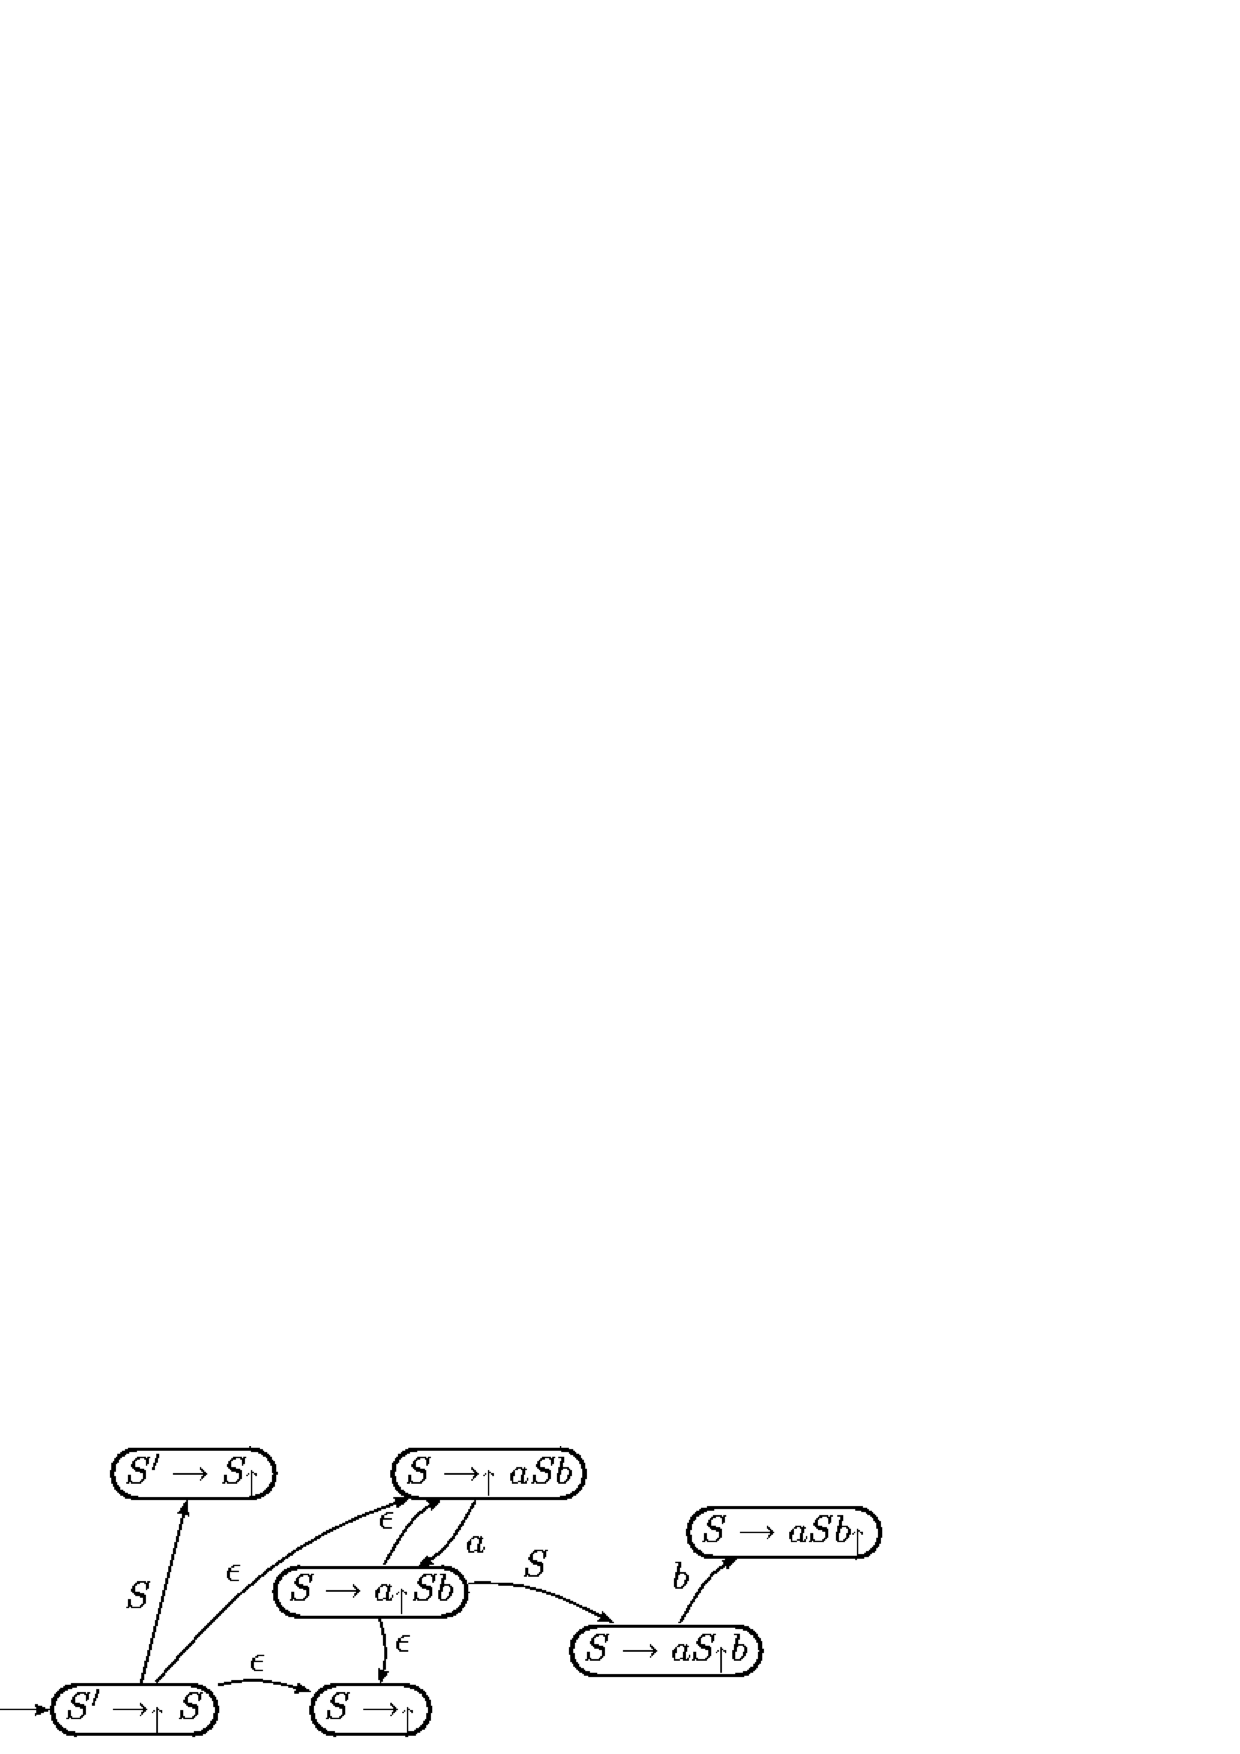
\includegraphics[scale=1.2]{chapter_bottomup/nfa.png}}
%\caption{NFA que reconoce los prefijos viables}
%\label{fig:nfa}
%\end{figure}
%\end{makeimage}
%\end{center}

\begin{center}
\begin{figure}[htb]
\centerline{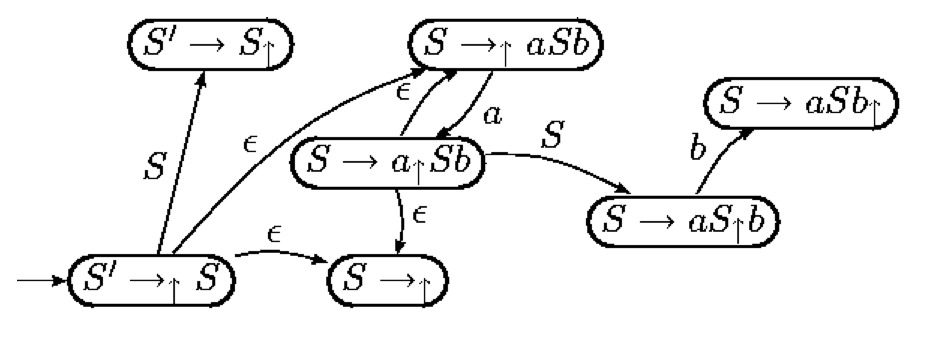
\epsfig{file=chapter_bottomup/nfa.eps, width=12cm}}
\caption{NFA que reconoce los prefijos viables}
\label{fig:nfa}
\end{figure}
\end{center}
\end{example}

\begin{exercise}
Simule el comportamiento del autómata sobre la entrada $aabb$. ¿Donde rechaza?
¿En que estados está el autómata en el momento del rechazo?. ¿Qué etiquetas tienen?
Haga también las
trazas del autómata para las entradas $aaSbb$ y $aSb$. ¿Que antiderivación 
ha construido el autómata con sus sucesivos rechazos? ¿Que terminales
se puede esperar que hayan en la entrada cuando se produce el rechazo
del autómata?
\end{exercise}

\section{Construcción de las Tablas para el Análisis SLR}

\subsection{Los conjuntos de Primeros y Siguientes}
\label{subsection:first}
Repasemos las nociones de conjuntos de \cei{Primeros} y \cei{siguientes}:

\begin{definition}
Dada una gramática $G=(\Sigma,V,P,S)$ y una frase $\alpha \in (V \cup \Sigma)^*$ se define el conjunto $FIRST(\alpha)$ como:

$FIRST(\alpha) = \left \{ b \in \Sigma :  \alpha  \stackrel{*}{\Longrightarrow}  b \beta \right \}
\cup N(\alpha)$ 

\noindent donde:

$N(\alpha) = \left \{ \begin{array}{ll}
                         \left \{ \epsilon \right \}& \mbox{si $\alpha \stackrel{*}{\Longrightarrow} \epsilon$} \\
                         \emptyset & \mbox{en otro caso} 
                      \end{array}
             \right. $ 

\end{definition}

\begin{definition}
Dada una gramática $G=(\Sigma,V,P,S)$ y una variable $A \in V$ se define el conjunto $FOLLOW(A)$ como: 

$FOLLOW(A) = \left \{ b \in \Sigma :  \exists\ S  \stackrel{*}{\Longrightarrow}  \alpha A b \beta \right \} \cup E(A)$

\noindent donde

$E(A) = \left \{ \begin{array}{ll}
                         \{ \$  \}& \mbox{si $S \stackrel{*}{\Longrightarrow} \alpha A$} \\
                         \emptyset & \mbox{en otro caso} 
                      \end{array}
             \right. $ 

\end{definition}

\begin{algorithm} Construcción de los conjuntos $FIRST(X)$
\begin{enumerate}
\item
$Si\ X \in \Sigma\ entonces\ FIRST(X) = {X}$
\item
$Si\ X \rightarrow \epsilon\ entonces\ FIRST(X) =  FIRST(X) \cup \{ \epsilon \}$
\item
$Si\ X \in V \ y\ X \rightarrow Y_1 Y_2 \cdots Y_k \in P\ entonces$
\begin{eqnarray*}
&&i = 1; \\
&&do\\
&&\ \ FIRST(X) = FIRST(X) \cup FIRST(Y_i) - \{ \epsilon \};\\
&&\ \ i++;\\
&&mientras\ (\epsilon \in FIRST(Y_i)\ and\ (i \leq k))\\
&&si\ (\epsilon \in FIRST(Y_k)\ and\ i > k)\ FIRST(X) = FIRST(X) \cup \{ \epsilon \}
\end{eqnarray*}
\end{enumerate}
\end{algorithm}
Este algoritmo puede ser extendido para calcular $FIRST(\alpha)$ para $\alpha = X_1 X_2 \cdots X_n \in (V \cup \Sigma)^*$.

\begin{algorithm} Construcción del conjunto $FIRST(\alpha)$ 
\begin{eqnarray*}
&&i = 1; \nonumber\\
&&FIRST(\alpha) = \emptyset; \nonumber\\
&&do \nonumber\\
&&\ \ FIRST(\alpha) = FIRST(\alpha) \cup FIRST(X_i) - \{ \epsilon \}; \nonumber\\
&&\ \ i++; \nonumber\\
&&mientras\ (\epsilon \in FIRST(X_i)\ and\ (i \leq n)) \nonumber\\
&&si\ (\epsilon \in FIRST(X_n)\ and\ i > n)\ FIRST(\alpha) = FIRST(X) \cup \{ \epsilon \}
\end{eqnarray*}
\end{algorithm} 

\begin{algorithm} Construcción de los conjuntos $FOLLOW(A)$
para las variables sintácticas $A \in V$: 

Repetir los siguientes pasos hasta que ninguno de los conjuntos $FOLLOW$ cambie:
\begin{enumerate} 
\item 
$FOLLOW(S) = \{\$\} $  ($\$$ representa el final de la entrada)
\item
$Si\ A \rightarrow \alpha B \beta\ entonces$
\[ FOLLOW(B) =  FOLLOW(B) \cup (FIRST(\beta) - \{\epsilon\})\]
\item
$Si\ A \rightarrow \alpha B$ o bien $A \rightarrow \alpha B \beta$
y $\epsilon \in FIRST(\beta)$  entonces

\[ FOLLOW(B) = FOLLOW(B) \cup FOLLOW(A)\]
\end{enumerate}
\end{algorithm}

\subsection{Construcción de las Tablas}
\label{subsection:nfa2dfa}

Para la construcción de las tablas de un analizador SLR
se construye el \cei{autómata finito determinista} (\cei{DFA}) 
$(Q, \Sigma, \delta, q_0)$ equivalente al NFA 
presentado en la sección
\ref{section:conceptosbasicos}
usando el \cei{algoritmo de construcción del subconjunto}.

Como recordará, en la construcción del subconjunto,
partiendo del estado de arranque $q_0$ del NFA con $\epsilon$-transiciones
se calcula su \cei{clausura} $\overline{\{q_0\}}$ y las 
clausuras de los conjuntos de estados $\overline{\delta(\overline{\{q_0\}},a)}$ 
a los que transita.  Se repite el proceso
con los conjuntos resultantes hasta que no se introducen nuevos
conjuntos-estado.

La clausura $\overline{A}$ de un subconjunto de estados del autómata $A$ esta formada
por todos los estados que pueden ser alcanzados mediante transiciones
etiquetadas con la palabra vacía (denominadas $\epsilon$ transiciones)
desde los estados de $A$. Se incluyen en $\overline{A}$, naturalmente los estados 
de $A$.

\begin{center}
$\overline{A} = \{ q \in Q\ /\  \exists q' \in Q\ :\ \hat{\delta}(q', \epsilon) = q \}$
\end{center}

Aquí $\hat{\delta}$ denota la \cei{función de transición del autómata} extendida  a cadenas
de $\Sigma^*$.

\begin{equation}
\label{equation:deltahat}
\hat{\delta}(q, x) = \left \{ \begin{array}{ll}
                         \delta(\hat{\delta}(q,y),a) & \mbox{si $x = ya$} \\
                         q & \mbox{si $x = \epsilon$} 
                      \end{array}
             \right.  
\end{equation}

En la práctica, y a partir de ahora así lo haremos, se prescinde de diferenciar
entre $\delta$ y $\hat{\delta}$ usándose indistintamente la notación
$\delta$ para ambas funciones.

La clausura puede ser computada usando una estructura de pila o aplicando 
la expresión recursiva dada en la ecuación \ref{equation:deltahat}.

Para el NFA mostrado en el ejemplo \ref{example:asb} el DFA construído mediante esta
técnica es el que se muestra en la figura \ref{fig:dfa}. Se ha utilizado el símbolo
\verb|#| como marcador. Se ha omitido el número 3 para que los estados coincidan
en numeración con los generados por \verb|jison| (véase el cuadro
\ref{table:tablaslalr}).

\begin{center}
\begin{figure}[htb]
%\centerline{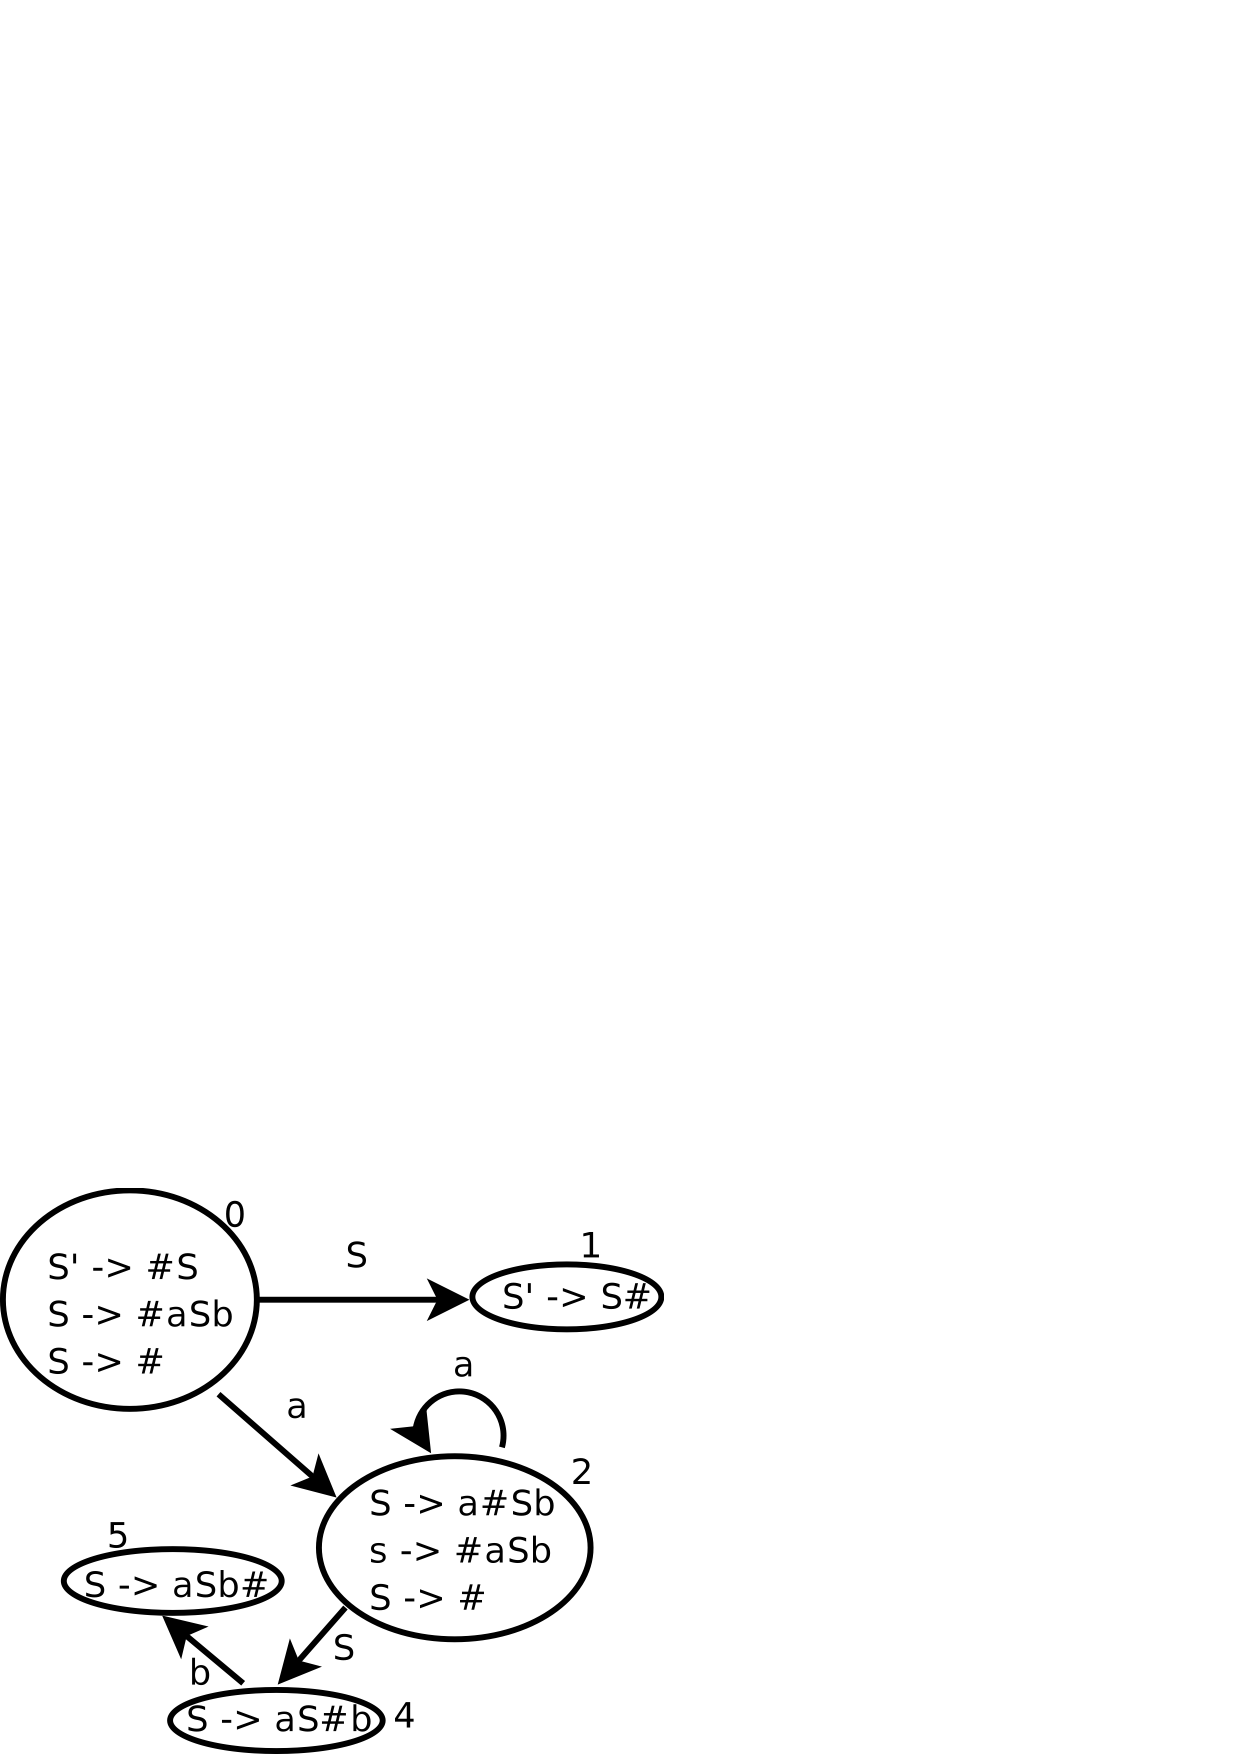
\includegraphics[scale=1.2]{chapter_bottomup/dfa.png}}
\centerline{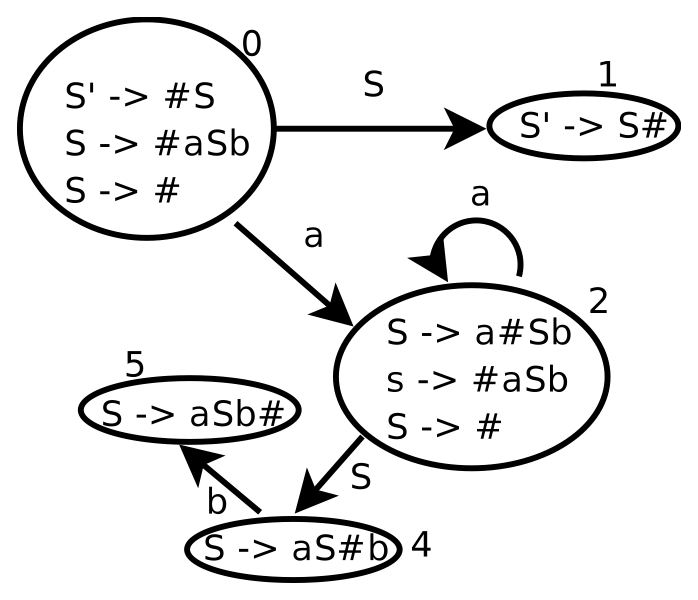
\epsfig{file=chapter_bottomup/dfa.eps, width=12cm}}
\caption{DFA equivalente al NFA de la figura \ref{fig:nfa}}
\label{fig:dfa}
\end{figure}
\end{center}

Un analizador sintáctico LR utiliza una tabla para su análisis.
Esa tabla se construye a partir de la tabla de transiciones del DFA.
De hecho, la tabla se divide en dos tablas, una llamada 
\cei{tabla de saltos} o \cei{tabla de gotos} y la otra
\cei{tabla de acciones}.

La tabla \cei{goto} de un analizador \cei{SLR}
no es más que la tabla de transiciones del autómata DFA 
obtenido aplicando la construcción del subconjunto al NFA
definido en \ref{definition:slrautomata}. De hecho es la tabla
de transiciones restringida a $V$ (recuerde que el alfabeto del
autómata es $V \cup \Sigma$, $i$ denota al i-ésimo estado resultante
de aplicar la construcción del subconjunto y que $I_i$ denota al conjunto de LR(0)
item asociado con dicho estado):

\begin{center}
$\delta_{| V \times Q} :  V \times Q \rightarrow Q$. 

donde se define $goto(i, A) = \delta(A,I_i)$
\end{center}

La parte de la función de transiciones
del DFA que corresponde a los terminales que no producen rechazo, 
esto es, $\delta_{| \Sigma \times Q} :  \Sigma \times Q \rightarrow Q$
se adjunta a una tabla que se denomina \cei{tabla de acciones}.
La tabla de acciones es una tabla de doble entrada en los estados
y en los símbolos de $\Sigma$.
Las acciones de transición ante terminales 
se denominan \cei{acciones de desplazamiento} o (\cei{acciones shift}):

\begin{center}
$\delta_{| \Sigma \times Q} :  \Sigma \times Q \rightarrow Q$

donde se define $action(i, a) = shift\ \delta(a,I_i)$
\end{center}

Cuando un estado $s$ contiene un LR(0)-item de la forma 
$A \rightarrow \alpha_\uparrow$, 
esto es, el estado corresponde a un posible rechazo,
ello indica que hemos llegado a un final del prefijo viable, que hemos
visto $\alpha$ y que, por tanto, es probable que $A \rightarrow \alpha$
sea el \emph{handle} de la forma sentencial derecha actual. Por tanto,
añadiremos en entradas de la forma $(s,a)$ de la tabla de acciones 
una acción que indique que hemos encontrado el mango en la 
posición actual y que la regla asociada es $A \rightarrow \alpha$.
A una acción de este tipo se la denomina \cei{acción de reducción}.

La cuestión es, ¿para que valores de $a \in \Sigma$ debemos disponer que
la acción para $(s, a)$ es de reducción?

\begin{center}
Se define $action(i, a) = reduce\ A \rightarrow \alpha$ ¿Pero, para que $a \in \Sigma$?
\end{center}


Podríamos decidir que ante cualquier terminal $a \in \Sigma$
que produzca un rechazo del autómata, pero podemos ser un poco mas
selectivos. No cualquier terminal puede estar en la entrada en el momento
en el que se produce la antiderivación o reducción. 
Observemos que si $A \rightarrow \alpha$ es el \emph{handle}
de $\gamma$ es porque:

\begin{center}
$\exists S \begin{array}{c} *\\ \Longrightarrow \\ {\scriptstyle RM} \end{array} \beta A b x \begin{array}{c} *\\ \Longrightarrow \\ {\scriptstyle RM} \end{array}  
\beta \alpha b x = \gamma$
\end{center}

Por tanto, cuando estamos reduciendo por $A \rightarrow \alpha$
los únicos terminales legales que cabe esperar en una reducción por $A \rightarrow \alpha$ son los terminales $b \in FOLLOW(A)$.

\begin{center}
Se define $action(i, b) = reduce\ A \rightarrow \alpha$ Para $b \in FOLLOW(A)$
\end{center}

Dada una gramática $G=(\Sigma,V,P,S)$, podemos construir las tablas de acciones (\emph{action table}) y  transiciones (\emph{gotos table}) mediante el siguiente algoritmo:

\begin{algorithm} 
\label{alg:tables}       
Construcción de Tablas \cei{SLR}

\begin{enumerate}
\item
Utilizando el Algoritmo de Construcción del Subconjunto, se construye
el Autómata Finito Determinista (DFA) $(Q, V \cup \Sigma, \delta, I_0, F)$
equivalente al Autómata Finito No
Determinista (NFA) definido en \ref{definition:slrautomata}.
Sea $C = \left \{ I_1, I_2, \cdots I_n \right \}$ el conjunto de estados
del DFA. Cada estado $I_i$ es un conjunto de LR(0)-items o estados
del NFA. Asociemos un índice $i$ con cada conjunto $I_i$.
\item
La tabla de \emph{gotos} no es más que la función de transición del 
autómata restringida a las variables de la gramática:

\begin{center}
$goto(i,A) = \delta(I_i, A)$ para todo $A \in V$
\end{center}
\item
Las acciones para el estado $I_i$ se determinan como sigue:
  \begin{enumerate}
  \item
  Si $A \rightarrow \alpha _\uparrow a \beta \in I_i$, $\delta(I_i,a) = I_j$, $a \in \Sigma$ 
  entonces:

\begin{center}
  $action[i][a] = shift\ j$
\end{center}
  \item
  Si $S' \rightarrow S_\uparrow \in I_i$ entonces 

\begin{center}
  $action[i][\$] = accept$
\end{center}
  \item
  Para cualquier otro caso de la forma $A \rightarrow \alpha _\uparrow \in I_i$ 
  distinto del anterior hacer

\begin{center}
  $\forall a \in\ FOLLOW(A):\ action[i][a] = reduce\ A \rightarrow \alpha$
\end{center}
  \end{enumerate}
\item
  Las entradas de la tabla de acción que queden indefinidas después de aplicado el proceso anterior corresponden a acciones de ``$error$''.
\end{enumerate}
\end{algorithm}

\begin{definition}
Si alguna de las entradas de la tabla resulta multievaluada, decimos
que existe un conflicto y que la gramática no es \cei{SLR}.

\begin{enumerate}
\item
En tal caso, si una de las acciones es de `reducción'' y la otra es de
`desplazamiento'', decimos que hay un \cei{conflicto shift-reduce} o
\cei{conflicto de desplazamiento-reducción}. 
\item
Si las
dos reglas indican una acción de reducción, decimos que tenemos un 
\cei{conflicto reduce-reduce} o de \cei{reducción-reducción}.
\end{enumerate}
\end{definition}

\begin{example}
\label{example:tablasslr}
Al aplicar el algoritmo \ref{alg:tables}       
a la gramática \ref{example:asb} 

\vspace{0.5cm}
\begin{center}
\begin{tabular}{|l|l|}
\hline
1 & S      $\rightarrow$  a S b\\
\hline
2 & S      $\rightarrow$ $\epsilon$ \\
\hline
\end{tabular}
\end{center}
\vspace{0.25cm}

partiendo del autómata finito determinista
que se construyó en 
la figura \ref{fig:dfa} y calculando los 
conjuntos de primeros y siguientes

\begin{center}
\begin{tabular}{|l|l|l|}
\hline
     & FIRST  & FOLLOW \\
\hline
S    & a, $\epsilon$ & b, \$\\
\hline
\end{tabular}
\end{center}

obtenemos la siguiente tabla de acciones SLR:

\begin{center}
\begin{tabular}{|l|l|l|l|}
\hline
     &  a  &  b  & \$ \\
\hline
0    & s2  &  r2 & r2 \\
\hline
1    &     &     & aceptar\\
\hline
2    & s2  & r2  & r2\\
\hline
4    &     & s5  &   \\
\hline
5    &     & r1  & r1\\
\hline
\end{tabular}
\end{center}

Las entradas denotadas con $s$ $n$ ($s$ por shift) indican un desplazamiento
al estado $n$, las denotadas con $r$ $n$ ($r$ por reduce o reducción) indican una operación
de reducción o antiderivación por la regla $n$.  Las entradas vacías 
corresponden a acciones de error.
\end{example}

El método de análisis \cei{LALR} usado por \verb|jison|
es una extensión del método SLR esbozado
aqui. Supone un compromiso entre potencia (conjunto de gramáticas
englobadas) y eficiencia (cantidad de memoria utilizada, tiempo de
proceso).
Veamos como \verb|jison| aplica la construcción del subconjunto a la 
gramática del ejemplo
\ref{example:asb}.
Para ello construimos el siguiente programa \verb|jison|:
\begin{verbatim}
[~/srcPLgrado/aSb(develop)]$ cat -n aSb.jison 
     1  %lex
     2  %%
     3  .               { return yytext; }
     4  /lex
     5  %%
     6  P: S            { return $1; }
     7  ;
     8  S: /* empty */  { console.log("empty");    $$ = ''; }
     9     | 'a' S 'b'  { console.log("S -> aSb"); $$ = $1+$2+$3; }
    10  ;
    11  %%
\end{verbatim}
y lo compilamos con \verb|jison|. Estas son las opciones disponibles:
\begin{verbatim}
nereida:[~/PLgradoBOOK(eps)]$ jison --help

Usage: jison [file] [lexfile] [options]

file        file containing a grammar
lexfile     file containing a lexical grammar

Options:
   -o FILE, --outfile FILE       Filename and base module name of the generated parser
   -t, --debug                   Debug mode
   -t TYPE, --module-type TYPE   The type of module to generate (commonjs, amd, js)
   -V, --version                 print version and exit
\end{verbatim}
Desafortunadamente carece de la típica opción \verb|-v| que permite generar las tablas
de análisis. Podemos intentar usar \verb|bison|, pero, obviamente, \verb|bison| protesta ante la entrada:

\begin{verbatim}
[~/srcPLgrado/aSb(develop)]$ bison -v aSb.jison 
aSb.jison:1.1-4: invalid directive: `%lex'
aSb.jison:3.1: syntax error, unexpected identifier
aSb.jison:4.1: invalid character: `/'
\end{verbatim}
El error es causado por la presencia del analizador léxico 
empotrado en el fichero \verb|aSb.jison|.  Si suprimimos provisionalmente
las líneas del analizador léxico empotrado,
\verb|bison| es capaz de analizar la gramática:
\begin{verbatim}
[~/srcPLgrado/aSb(develop)]$ bison -v aSb.jison 
[~/srcPLgrado/aSb(develop)]$ ls -ltr | tail -1
-rw-rw-r--  1 casiano  staff    926 19 mar 13:29 aSb.output
\end{verbatim}
Que tiene los siguientes contenidos:
\begin{verbatim}
[~/srcPLgrado/aSb(develop)]$ cat -n aSb.output 
     1  Grammar
     2  
     3      0 $accept: P $end
     4  
     5      1 P: S
     6  
     7      2 S: /* empty */
     8      3  | 'a' S 'b'
     9  
    10  
    11  Terminals, with rules where they appear
    12  
    13  $end (0) 0
    14  'a' (97) 3
    15  'b' (98) 3
    16  error (256)
    17  
    18  
    19  Nonterminals, with rules where they appear
    20  
    21  $accept (5)
    22      on left: 0
    23  P (6)
    24      on left: 1, on right: 0
    25  S (7)
    26      on left: 2 3, on right: 1 3
    27  
    28  
    29  state 0
    30  
    31      0 $accept: . P $end
    32  
    33      'a'  shift, and go to state 1
    34  
    35      $default  reduce using rule 2 (S)
    36  
    37      P  go to state 2
    38      S  go to state 3
    39  
    40  
    41  state 1
    42  
    43      3 S: 'a' . S 'b'
    44  
    45      'a'  shift, and go to state 1
    46  
    47      $default  reduce using rule 2 (S)
    48  
    49      S  go to state 4
    50  
    51  
    52  state 2
    53  
    54      0 $accept: P . $end
    55  
    56      $end  shift, and go to state 5
    57  
    58  
    59  state 3
    60  
    61      1 P: S .
    62  
    63      $default  reduce using rule 1 (P)
    64  
    65  
    66  state 4
    67  
    68      3 S: 'a' S . 'b'
    69  
    70      'b'  shift, and go to state 6
    71  
    72  
    73  state 5
    74  
    75      0 $accept: P $end .
    76  
    77      $default  accept
    78  
    79  
    80  state 6
    81  
    82      3 S: 'a' S 'b' .
    83  
    84      $default  reduce using rule 3 (S)
\end{verbatim}

Observe que el final de la entrada se denota 
por \verb|$end| y el marcador en un LR-item 
por un punto. Fíjese en el estado 1: 
En ese estado están también los items

\begin{center}
 \verb|S -> . 'a' S 'b'|
y \verb|S -> .|
\end{center}

sin embargo no se explicitan
por que se entiende que su pertenencia es
consecuencia directa de aplicar la operación 
de clausura. Los LR items cuyo marcador
no está al principio se denominan
\cei{items núcleo}. 

\sectionpractica{Analizador de PL0 Usando Jison}
\label{practica:pl0ampliadojison}
Reescriba el analizador sintáctico del lenguaje PL0 
realizado en las prácticas
\ref{practica:pl0}
y
\ref{practica:pl0ampliado}
usando \jison{}.

\parrafo{Donde}

\begin{itemize}
\item
\htmladdnormallink{Repositorio en GitHub}{https://github.com/crguezl/ull-etsii-grado-pl-jisoncalc}
\item
\htmladdnormallink{Despliegue en Heroku}{http://jisoncalc.herokuapp.com/}
\item
\begin{verbatim}
[~/jison/jisoncalc(develop)]$ pwd -P
/Users/casiano/local/src/javascript/PLgrado/jison/jisoncalc
\end{verbatim}
\item
\begin{verbatim}
[~/jison/jisoncalc(develop)]$ git remote -v
heroku  git@heroku.com:jisoncalc.git (fetch)
heroku  git@heroku.com:jisoncalc.git (push)
origin  git@github.com:crguezl/ull-etsii-grado-pl-jisoncalc.git (fetch)
origin  git@github.com:crguezl/ull-etsii-grado-pl-jisoncalc.git (push)
\end{verbatim}
\end{itemize}

\parrafo{Tareas}
\begin{itemize}
\item
La salida debe ser el AST del programa de entrada
\item
Modifique \verb|block| y \verb|statement| para que los 
\verb|procedure| reciban argumentos y las llamadas 
a procedimiento puedan pasar argumentos.
\item
Añada \verb|if ... then ... else ...|.
\item Actualice la documentación de la gramática para que refleje la gramática ampliada
\item
Limite el número de programas que se pueden salvar a un número prefijado, por ejemplo 10. Si se intenta salvar uno se suprime uno al azar y se guarda el nuevo.
\item
Las pruebas deben comprobar que los AST generados reflejan la semántica
del lenguaje así como alguna situación de error
\item
Sólo usuarios autenticados pueden salvar sus programas en la base de datos.
\item
Extienda la autenticación \OAuth{} para que además de Google pueda hacerse
con Twitter ó GitHub ó Facebook ó ... Sólo debe implementar una.
\item Método de Entrega:
\begin{itemize}
\item
Use un repositorio 
privado en BitBucket o bien solicite al administrador del Centro de Cálculo 
un repositorio privado en GitHub.
\item
Comparta dicho repositorio con sus colaboradores y con el profesor.
\item
Suba la práctica al workshop/taller antes de la fecha límite
\item
Cuando el taller pase a la fase de evaluación haga público su repositorio
\end{itemize}
\end{itemize}

\parrafo{Referencias para esta Práctica}
\begin{itemize}
\item Véase el capítulo 
{\it Oauth: Google, Twitter, GitHub, Facebook}
\ref{chapter:googleoauth}
\item Véase 
\htmladdnormallink{Intridea Omniauth}{http://intridea.github.io/omniauth/}
y
\htmladdnormallink{omniauth en GitHub}{https://github.com/intridea/omniauth}
\item
La gema \htmladdnormallink{omniauth-google-oauth2}{https://github.com/zquestz/omniauth-google-oauth2}
\item
\htmladdnormallink{Google Developers Console}{https://console.developers.google.com/project}
\item
\htmladdnormallink{Revoking Access to an App in Google}{https://security.google.com/settings/security/permissions?pli=1}
\item
La gema 
\htmladdnormallink{sinatra-flash}{https://github.com/SFEley/sinatra-flash}
\item Véase el capítulo {\it Heroku} \ref{chapter:heroku}
\item
\htmladdnormallink{Heroku Postgres}{https://devcenter.heroku.com/articles/heroku-postgresql}
\item Véase el capítulo {\it DataMapper} \ref{chapter:datamapper}
\end{itemize}

\sectionpractica{Análisis de Ámbito en PL0}
\label{practica:analisisdeambitopl0}
\parrafo{Objetivos}

\begin{itemize}
\item
Modifique la práctica anterior para que cada nodo del tipo \verb|PROCEDURE|
disponga de una tabla de símbolos en la que se almacenan todos las
constantes, variables  y procedimientos declarados en el mismo.

\item
Existirá ademas una tabla de símbolos asociada con el nodo raíz 
que representa al programa principal.
\item
Las declaraciones de constantes y variables no crean nodo, sino que se
incorporan como información a la tabla de símbolos del procedimiento
actual
\item
Para una entrada de la tabla de símbolos
\verb|sym["a"]| se guarda que clase de objeto
es: constante, variable, procedimiento, etc.
\item
Si es un procedimiento se guarda el número de argumentos
\item
Si es una constante se guarda su valor
\item 
Cada uso de un identificador (constante, variable, procedimiento)
tiene un atributo \verb|declared_in| que referencia en que nodo
se declaró
\item
Si un identificador es usado y no fué declarado es un error
\item
Si se trata de una llamada a procedimiento (se ha usado \verb|CALL| y el identificador corresponde a un \verb|PROCEDURE|)
se comprobará que el número 
de argumentos coincide con el número de parámetros declarados en su 
definición
\item
Si es un identificador de una constante, es un error
que sea usado en la parte
izquierda de una asignación (que no sea la de su declaración)
\item Base de Datos
\begin{enumerate}
\item
Guarde en una tabla el nombre de usuario que guardó un programa.
Provea una ruta para ver los programas de un usuario.
\item
Un programa \verb|belongs_to| un usuario. Un usuario \verb|has n| programas.
Vea la sección
\htmladdnormallink{DataMapper Associations}{http://datamapper.org/docs/associations.html}.
\end{enumerate}
\item
Use la sección \verb|issues| de su repositorio en 
GitHub para coordinarse así como
para llevar un histórico de las incidencias y la forma en la que
se resolvieron. Repase el tutorial
\htmladdnormallink{Mastering Issues}{https://guides.github.com/overviews/issues/}

\end{itemize}


\sectionpractica{Traducción de Infijo a Postfijo}
\label{section:calculadoraampliada}
Modifique el programa Jison realizado en la práctica 
\ref{subsectionpractica:calculadora}
para traducir de infijo a postfijo. 
Añada los operadores de comparación e igualdad.
Por ejemplo

\begin{center}
\begin{tabular}{p{6cm}|p{6cm}}
Infijo              & Postfijo \\
\verb|a = 3+2*4|    &  \verb| 3 2 4 * + &a = |\\
\verb|b = a == 11|  &  \verb| a 11 == &b = |
\end{tabular}
\end{center}
En estas traducciones la notación 
\verb|&a| indica la dirección de la variable \verb|a|
y \verb|a| indica el valor almacenado en la variable \verb|a|.

Añada sentencias 
\verb|if| ...
\verb|then| e \verb|if| ... \verb|then| ... \verb|else|

Para realizar la traducción de estas sentencias
añada 
instrucciones \verb|jmp label| y \verb|jmpz label| (por {\it jump if zero})
y etiquetas:

\begin{center}
\begin{tabular}{p{8cm}|p{6cm}}
Infijo              & Postfijo \\
\begin{verbatim}
a = (2+5)*3;
if a == 0 then b = 5 else b = 3;
c = b + 1;
\end{verbatim}
&
\begin{verbatim}
        2
        5
        +
        3
        *
        &a
        =
        a
        0
        ==
        jmpz else1
        5
        &b
        =
        jmp endif0
:else1
        3
        &b
        =
:endif0
        b
        1
        +
        &c
        =
\end{verbatim}
\end{tabular}
\end{center}
Parta del repositorio 
\htmladdnormallink{https://github.com/crguezl/jison-simple-html-calc}{https://github.com/crguezl/jison-simple-html-calc}.

%Introduzca pruebas unitarias como las descritas en 
%la sección \ref{section:tstingfacil} ({\it
%\htmladdnormallink{Quick Tip: Quick and Easy JavaScript Testing with “Assert”}{http://net.tutsplus.com/tutorials/javascript-ajax/quick-tip-quick-and-easy-javascript-testing-with-assert/}})
%
%\begin{verbatim}
%[~/srcPLgrado/jisoninfix2postfix(master)]$ cat test/test.html 
%<!DOCTYPE HTML>
%<html lang="en">
%  <head>
%    <meta charset="UTF-8">
%    <title>Testing Our Simple Translator</title>
%    <link rel="stylesheet" href="test.css" />
%    <script type="text/javascript" src="../calculator.js"></script>
%
%  </head>
%  <body>
%    <h1>Testing Our Simple Translator
%    </h1>
%    
%    <ul id="output"></ul>
%    <script type="text/javascript" src="assert.js"></script>
%    
%    <script type="text/javascript">
%
%      var r = calculator.parse("a = 4*8");
%      assert( /4\s*8\s*[*]\s*a\s*=\s*/.exec(r), "a is 4*8");
%      
%      r = calculator.parse("a=4;b=a+1");
%      r = r.replace(/\s+/g,'');
%      var expected = "4a=a1+b=";
%      assert( r == expected, "a = 4;\nb=a+1 translated");
%
%
%      var r = calculator.parse("if a > 0 then b = 1 else b = 2");
%      r = r.replace(/\s+/g,'');
%      expected = "a 0 > jmpz else1 1 b = jmp endif0 :else1 2 b = :endif0".
%                 replace(/\s+/g,'');
%      assert( r == expected, "'if a > 0 then b = 1 else b = 2' translated");
%    </script>
%      See the NetTuts+ tutorial at <a href="http://net.tutsplus.com/tutorials/javascript-ajax/quick-tip-quick-and-easy-javascript-testing-with-assert/">Quick and Easy JavaScript Testing</a>
%  </body>
%</html>
%\end{verbatim}

\sectionpractica{Calculadora  con Funciones}

Añada funciones y sentencias de llamada a función a la práctica de traducción 
de infijo a postfijo
\ref{section:calculadoraampliada}. Sigue un ejemplo de traducción:

\begin{tabular}{|p{6cm}|p{6cm}|}
\hline
\begin{verbatim}
def f(x) { x + 1 }
def g(a, b) { a * f(b) }
c = 3;
f(1+c);
g(3, 4)
\end{verbatim}
&
\begin{verbatim}
:f      args :x
        $x
        1
        +
        return
:g      args :a,:b
        $a
        $b
        call :f
        *
        return
:main:
        3
        &c
        =
        1
        c
        +
        call :f
        3
        4
        call :g
\end{verbatim}
\end{tabular}
\begin{itemize}
\item
Las funciones retornan la última expresión evaluada
\item
Es un error llamar a una función con un número de argumentos 
distinto que el número de parámetros con el que fué declarada
\item
En la llamada, los argumentos se empujan en la pila.
Después la instrucción \verb|call :etiqueta| llama a
la función con el nombre dado por la \verb|etiqueta|
\item
Dentro de la función los argumentos se sitúan por encima del puntero 
base. La pseudo-instrucción \verb|args, p1, p2, ...| da nombre a los 
parámetros empujados. Dentro del cuerpo de la función nos referimos a ellos
prefijándolos con \verb|$|.
\item
La instrucción \verb|return| limpia la pila dejándola en su estado anterior 
y retorna la última expresión evaluada
\end{itemize}

\sectionpractica{Calculadora con Análisis de Ámbito}
\label{practica:ambitocalc}
Extienda la práctica anterior para que haga un análisis completo del ámbito de las variables.

\begin{itemize}
\item Añada declaraciones de variable con \verb|var x, y = 1, z|.
Las variables podrán opcionalmente ser inicializadas.
Se considerará un error usar una variable no declarada.
\item
Modifique la gramática para que permita el anidamiento de funciones: funciones dentro de funciones.
\begin{verbatim}
var c = 4, d = 1, e;
def g(a, b) { 
  var d, e;
  def f(u, v) { a + u + v + d }
  a * f(b, 2) + d + c 
}
\end{verbatim}
\item
Una declaración de variable en un ámbito anidado tapa a una declaración con el mismo nombre en el ámbito exterior.

\begin{tabular}{|p{6cm}|p{6cm}|}
\hline
\begin{verbatim}
var c = 4, d = 1, e;
def g(a, b) { 
  var d, e; # esta "d" tapa la d anterior
  def f(u, v) { a + u + v + d }
  a * f(b, 2) + d + c 
}
\end{verbatim}
&
\begin{verbatim}
        # global:       var c,d,e
:g.f
        $a, 1
        $u, 0
        +
        $v, 0
        +
        d, 1
        +
        return
:g
        $a, 0
        $b, 0
        2
        call :g.f
        *
        d, 0     # acceder a la d en el ámbito actual
        +
        c, 1
        +
        return
\end{verbatim}\\
\hline
\end{tabular}

\item
Los nombres de funciones se traducen por una secuencia anidada de nombres
que indican su ámbito. 
Así la función \verb|f| anidada en \verb|g|
es traducida a la función con nombre \verb|g.f|.
Una función \verb|h| anidada en una función \verb|f| anidada en \verb|g|
es traducida a la función con nombre \verb|g.f.h|

\item Las variables ademas de su nombre (dirección/offset) reciben un entero adicional
0,1,2, \ldots que indica su nivel de anidamiento. El número de stack frames que hay que recorrer para llegar a la variable
\begin{verbatim}
        $a, 1
        $u, 0
        +
        $v, 0
        +
        d, 1
        +
\end{verbatim}
Asi \verb|$a, 1| significa acceder al parámetro \verb|a| que está a distancia 
\verb|1| del stack frame/ámbito actual y \verb|$v, 0| es el parámetro \verb|v|
en el ámbito/stack frame actual
\item El frame pointer o base pointer BP indica el nivel de anidamiento estático (en 
el fuente) de la rutina. Así cuando se va a buscar una variable local
declarada en la rutina que anida la actual se recorre la lista de frames via BP o frame pointer tantas veces como el nivel de anidamiento indique.


\begin{rawhtml}
<center>
<img src="stackframes.png" />
</center>
\end{rawhtml}
\item
\begin{enumerate}
\item
Esto es lo que dice la Wikipedia sobre la implementación de \wikip{llamadas}{call\_stack}
a subrutinas anidadas:
\begin{quote}
{\it
Programming languages that support nested subroutines also have a field
in the call frame that points to the stack frame of the latest activation
of the procedure that most closely encapsulates the callee, i.e. the
immediate scope of the callee. This is called an \cei{access link} or 
\cei{static link} (as it keeps track of static nesting during dynamic and recursive
calls) and provides the routine (as well as any other routines it may
invoke) access to the local data of its encapsulating routines at every
nesting level. 
}
\end{quote}
\item
Esto es lo que dice sobre las 
ventajas de tener una pila y de almacenar la dirección de retorno y las variables locales:
\begin{quote}
When a subroutine is called, the location (address) of the instruction at
which it can later resume needs to be saved somewhere. Using a stack to
save the return address has important advantages over alternatives. One
is that each task has its own stack, and thus the subroutine can be
\cei{reentrant}, that is, can be active simultaneously for different tasks doing
different things. Another benefit is that \cei{recursion} is automatically
supported. When a function calls itself recursively, a return address
needs to be stored for each activation of the function so that it can
later be used to return from the function activation. This capability
is automatic with a stack.
\end{quote}

\item Almacenamiento local:
\begin{quote}
A subroutine frequently needs memory space for storing the values of
local variables, the variables that are known only within the active
subroutine and do not retain values after it returns. It is often
convenient to allocate space for this use by simply moving the top of
the stack by enough to provide the space. This is very fast compared to
heap allocation. Note that each separate activation of a subroutine gets
its own separate space in the stack for locals.
\end{quote}


\item Parámetros:
\begin{quote}
Subroutines often require that values for parameters be supplied to
them by the code which calls them, and it is not uncommon that space for
these parameters may be laid out in the call stack. 

The call stack works well as a
place for these parameters, especially since each call to a subroutine,
which will have differing values for parameters, will be given separate
space on the call stack for those values.
\end{quote}

\item
Pila de Evaluación

\begin{quote}
Operands for arithmetic or logical operations are most often placed into
registers and operated on there. However, in some situations the operands
may be stacked up to an arbitrary depth, which means something more than
registers must be used (this is the case of \cei{register spilling}). The stack
of such operands, rather like that in an RPN calculator, is called an
\cei{evaluation stack}, and may occupy space in the call stack.
\end{quote}

\item
Puntero a la instancia actual
\begin{quote}
Some object-oriented languages (e.g., C++), store the \verb|this| pointer along
with function arguments in the call stack when invoking methods. The
\tei{this pointer} points to the object instance associated with the method
to be invoked.
\end{quote}
\end{enumerate}

\item Los parámetros se siguen prefijando de \verb|$| como en la práctica anterior
\item Sigue un ejemplo de traducción:
\begin{tabular}{|p{6cm}|p{6cm}|}
\hline
\begin{verbatim}
var c = 4, d = 1, e;
def f(x) { 
  var y = 1;
  x + y 
}
def g(a, b) { 
  var d, e;
  def f(u, v) { a + u + v + d }
  a * f(b, 2) + d + c 
}
c = 3;
f(1+c);
g(3, 4)
\end{verbatim}
&
\begin{verbatim}
        # global:       var c,d,e
        # f: args x
        # f:    var y
:f
        1
        &y, 0
        =
        $x, 0
        y, 0
        +
        return
        # g: args a,b
        # g:    var d,e
        # g.f: args u,v
:g.f
        $a, 1
        $u, 0
        +
        $v, 0
        +
        d, 1
        +
        return
:g
        $a, 0
        $b, 0
        2
        call :g.f
        *
        d, 0
        +
        c, 1
        +
        return
:main:
        4
        &c, 0
        =
        1
        &d, 0
        =
        3
        &c, 0
        =
        1
        c, 0
        +
        call :f
        3
        4
        call :g
\end{verbatim}\\
\hline
\end{tabular}

\item
Puede comenzar haciendo un fork del proyecto 
\htmladdnormallink{ull-etsii-grado-pl-infix2postfix}{https://github.com/crguezl/ull-etsii-grado-pl-infix2postfix}
en GitHub. Esta incompleto. Rellene las acciones semánticas que faltan;
la mayoría relacionadas con el análisis de ámbito.

\item
\begin{itemize}
\item
Una solución completa se encuentra en el proyecto
\htmladdnormallink{crguezl/jisoninfix2postfix}{https://github.com/crguezl/jisoninfix2postfix}.
\item
\begin{verbatim}
[~/jison/jisoninfix2postfix(gh-pages)]$ pwd -P
/Users/casiano/local/src/javascript/PLgrado/jison/jisoninfix2postfix
\end{verbatim}
\item
\begin{verbatim}
[~/jison/jisoninfix2postfix(gh-pages)]$ git remote -v
bitbucket       ssh://git@bitbucket.org/casiano/jisoninfix2postfix.git (fetch)
bitbucket       ssh://git@bitbucket.org/casiano/jisoninfix2postfix.git (push)
origin  git@github.com:crguezl/jisoninfix2postfix.git (fetch)
origin  git@github.com:crguezl/jisoninfix2postfix.git (push)
\end{verbatim}
\end{itemize}
\item
Veanse:
  \begin{itemize}
  \item
  Véase COMP 3290 Compiler Construction
  Fall 2008
  \htmladdnormallink{Notes/Symbol Tables}{http://www.cs.umanitoba.ca/~comp3290/Notes/05symboltable.pdf}
  \item
  El capítulo 
  \htmladdnormallink{Symbol Table
  Structure}{http://books.google.es/books?id=Pq7pHwG1_OkC} del libro de
  Muchnick Advanced Compiler Design Implementation \cite{Muchnick:1998:ACD:286076}
  \item
  El capítulo 
  \htmladdnormallink{Symbol Table
  Structure}{http://www.cs.umanitoba.ca/~comp3290/Docs/basics_letter_12pt.pdf} del libro de
  Basics of Compiler Design de Torben Ægidius Mogensen \cite{mogensen2011introduction}
  \end{itemize}
\end{itemize}

\section{Algoritmo de Análisis LR}
\label{section:algoritmoLR}
Asi  pues la tabla de transiciones del autómata nos genera dos tablas:
la tabla de acciones y la de saltos.
El  algoritmo  de análisis sintáctico \emph{LR} en el  que 
se basa \emph{jison} utiliza una pila y dos tablas 
para analizar la entrada. % (véase la figura \ref{fig:lrparser}). 
Como se ha visto, la tabla  de acciones contiene cuatro tipo de acciones: 
\begin{enumerate}
\item
Desplazar (\emph{shift})
\item
Reducir (\emph{reduce})
\item
Aceptar
\item
Error
\end{enumerate}
El algoritmo utiliza una pila en la que se guardan los estados
del autómata. De este modo se evita tener que ``comenzar'' 
el procesado de la forma sentencial derecha resultante
después de una reducción (antiderivación).
\begin{algorithm}
\label{alg:parser}       
Análizador LR
\begin{verbatim}
 push(s0);
 b = yylex();
 for( ; ; ;) {
   s = top(0); a = b;
   switch (action[s][a]) {
     case "shift t" : 
       t.attr = a.attr;
       push(t); 
       b = yylex();
       break;
     case "reduce A ->alpha" : 
       eval(Sem{A -> alpha}(top(|alpha|-1).attr, ... , top(0).attr)); 
       pop(|alpha|); 
       push(goto[top(0)][A]); 
       break;
     case "accept" : return (1); 
     default : yyerror("syntax error");
   }
 }
\end{verbatim}
\end{algorithm}
\begin{itemize}
\item
Como es habitual, $|x|$ denota la longitud de la cadena $x$.
\item
La función \verb|top(k)| devuelve el elemento que ocupa la 
posición \verb|k| desde el \emph{top} de la pila (esto es, está a profundidad \verb|k|).
\item
La función \verb|pop(k)| extrae \verb|k| elementos de la pila.
\item
La notación \verb|state.attr| hace referencia al atributo
asociado con cada estado, el cual desde el punto de vista del programador
esta asociado con el correspondiente símbolo de la parte derecha de la regla. 
Nótese que cada estado que está en la pila es el resultado de una transición con
un símbolo. El atributo de ese símbolo es guardado en el objeto estado
cada vez que ocurre una transición.

\item
Denotamos por \verb|Sem {reduce A -> alpha}|
el código de la acción semántica asociada con la regla $A \rightarrow \alpha$.
\end{itemize}
%\begin{figure}
%\input{parser_fig.tex}
%\caption{Estructura de un Análizador LR}
%\label{fig:lrparser}       
%\end{figure}

Todos los analizadores LR comparten, salvo pequeñas
excepciones, el mismo algoritmo
de análisis. Lo que más los diferencia es la forma en 
la que construyen las tablas.
En \verb|jison|
la construcción de las tablas de \emph{acciones} y \emph{gotos}
se realiza  por defecto mediante el algoritmo \emph{LALR}.


\section{El módulo Generado por {\tt jison}}
\label{section:tablas}

\subsection{Version}

En esta sección estudiamos el analizador generado por Jison:
\begin{verbatim}
[~/Dropbox/src/javascript/PLgrado/jison-aSb(develop)]$ jison --version
0.4.2
\end{verbatim}

\subsection{Gramática Inicial}
Veamos el módulo generado por jison para esta gramática:
\begin{verbatim}
[~/srcPLgrado/aSb(develop)]$ cat aSb.jison 
%lex
%%
.               { return yytext; }
/lex
%%
S: /* empty */  { console.log("empty"); }
   | 'a' S 'b'  { console.log("S -> aSb"); }
;
%%
\end{verbatim}

% edit chapter_bottomup/aSb.tex
\subsection{Tablas}
Esta es la primera parte del parser generado:
\begin{verbatim}
/* parser generated by jison 0.4.2 */
var aSb = (function() {
    var parser = {
        trace: function trace() {},
        yy: {},
        symbols_: {
            "$accept": 0, /* super-arranque $accept -> S */
            "$end": 1     /* end of input */
            "error": 2, /* numero para el símbolo 'error' */
            "S": 3,     /* numero para el símbolo 'S' */
            "a": 4,
            "b": 5,
        },
        /* array inverso de terminales */
        terminals_: {   /* numero -> terminal */
            2: "error", 
            4: "a",
            5: "b"
        },
        productions_: 
        [0, 
/* 1 */     [3, 0], /* S : vacio        simbolo,longitud de la parte derecha */
/* 2 */     [3, 3]  /* S : a S b        simbolo,longitud */
        ],
\end{verbatim}

\begin{center}
\begin{latexonly}
\begin{figure}[htb]
%\centerline{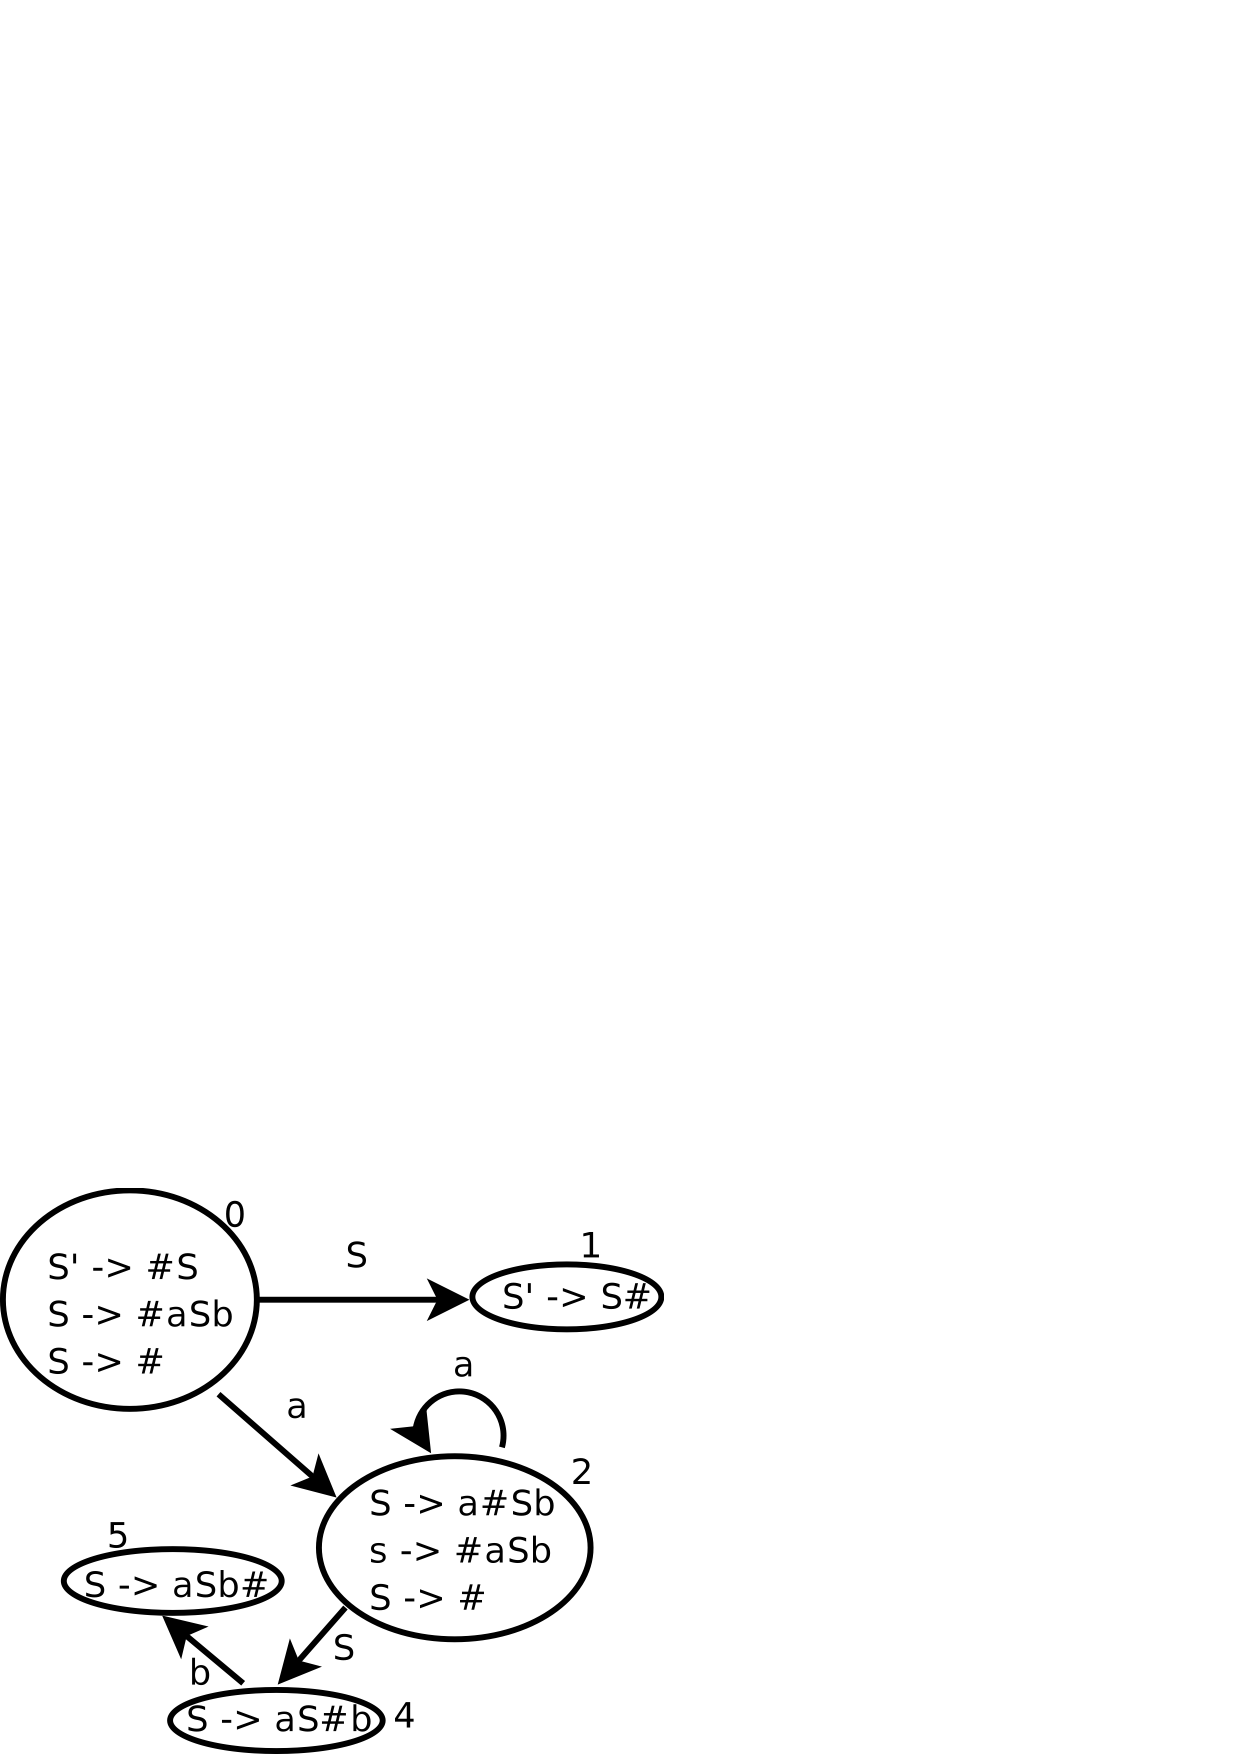
\includegraphics[scale=1.2]{chapter_bottomup/dfa.png}}
\centerline{\epsfig{file=chapter_bottomup/aSb.eps, width=12cm}}
\caption{DFA construido por Jison}
\label{fig:dfa}
\end{figure}
\end{latexonly}
\begin{rawhtml}
<img src="aSb.png" width="50%"/>
<p>

DFA construido por Jison
\end{rawhtml}
\end{center}

\subsection{Acciones Semánticas}
Cada vez que se produce una acción de reducción esta función es llamada:
\begin{verbatim}
performAction: function anonymous(yytext, yyleng, yylineno, yy, yystate, $$, _$) {

    var $0 = $$.length - 1;
    switch (yystate) { /* yystate: numero de regla de producción */
        case 1:
            console.log("empty");
            break;
        case 2:
            console.log("S -> aSb");
            break;
    }
},
\end{verbatim}
\begin{itemize}
\item
Parece que  cuando se llama a este método \verb|this| refiere a un objeto \verb|yyval|. Este es el
punto  de llamada a la acción semántica dentro del parser generado por Jison.
Puede encontrarse dentro del parser en el caso de un \verb|switch| 
que corresponde a la acción de reducción:
\begin{verbatim}
r = this.performAction.call(yyval, yytext, yyleng, yylineno, this.yy, action[1], vstack, lstack);
\end{verbatim}
El método \verb|call|
nos permite invocar una función como si fuera un método de algún otro 
objeto. Véase la sección 
\ref{subsection:callyapply}.

Este objeto \verb|yyval| tiene dos atributos: \verb|$| y \verb|_$|.
  \begin{itemize}
  \item
  El atributo 
  \verb|$| se corresponde con \verb|$$| de la gramática (atributo de la variable
  sintactica en la parte izquierda)
  \item
  El atributo \verb|_$| guarda información
  sobre la posición del último token leído.
  \end{itemize}
\item
\verb|yytext| parece contener el texto asociado con el token actual
\item
\verb|yyleng| es la longitud del token actual
\item
\verb|yylineno| es la línea actual (empezando en 0)
\item
\verb|yy| es un objeto con dos atributos \verb|lexer| y \verb|parser| 
\item
\verb|yystate| es el estado actual 
\item
\verb|$$| parece ser un array/pila conteniendo 
los valores de los atributos asociados con los estados de la pila (\verb|vstack| ¿Por value stack?)
\item
Asi pues \verb|$0| es el índice en \verb|$0| del último elemento de \verb|$$|.
Por ejemplo, una acción semántica asociada con una regla \verb|A : B C D| con tres elementos como:
\begin{verbatim}
$$ = $1 + $2 + $3;
\end{verbatim}
Se traduce por:
\begin{verbatim}
this.$ = $$[$0 - 2] + $$[$0 - 1] + $$[$0];
\end{verbatim}
\item
\verb|_$|
Es un array con la información sobre la localización de los simbolos (\verb|lstack| ¿Por location stack?)
\end{itemize}

\subsection{Tabla de Acciones y GOTOs}

\begin{verbatim}
        table: [{
/* 0 */     1: [2, 1],    /* En estado 0 viendo $end(1) reducir por S : vacio */
            3: 1,         /* En el estado 0 viendo S(3) ir al estado 1 */
            4: [1, 2]     /* Estado 0 viendo a(4) shift(1) al estado 2 */
        }, {
/* 1 */     1: [3]        /* En 1 viendo $end(1) aceptar */
        }, {
/* 2 */     3: 3,         /* En 2 viendo S ir a 3 */
            4: [1, 2],    /* En 2 viendo a(4) shift a 2 */
            5: [2, 1]     /* En 2 viendo b(5) reducir por regla 1: S -> vacio */
        }, {
/* 3 */     5: [1, 4]     /* En 3 viendo b(5) shift a 4 */
        }, {
/* 4 */     1: [2, 2],    /* En 4  viendo $end(1) reducir(2) por la 2: S -> aSb */
            5: [2, 2]     /* En 4 viendo b(5) reducir por la 2: S-> aSb */
        }],
\end{verbatim}

\begin{itemize}
\item
La tabla es un array de objetos
\item
El índice de la tabla es el estado. En el ejemplo tenemos 5 estados
\item
El objeto/hash que es el valor contiene las acciones ante los símbolos.
\begin{enumerate}
\item
Los atributos/claves son los símbolos, los valores las acciones
\item
Las acciones son de dos tipos:
\begin{enumerate}
\item
El número del estado al que se transita mediante la tabla \verb|goto|
cuando el símbolo es una variable sintactica 
\item
Un par \verb|[tipo de acción, estado o regla]|. 
Si el \verb|tipo de acción| es 1 indica un shift al \verb|estado| con ese número.
Si el \verb|tipo de acción| es 2 indica una reducción por la \verb|regla| con ese número.
\end{enumerate}
\item
Por ejemplo \verb|table[0]| es 
\begin{verbatim}
        {
            1: [2, 1],    /* En estado 0 viendo $end(1) reducir(2) por S : vacio */
            3: 1,         /* En el estado 0 viendo S(3) ir (goto) al estado 1 */
            4: [1, 2]     /* Estado 0 viendo a(4) shift(1) al estado 2 */
        } 
\end{verbatim}
\end{enumerate}


\end{itemize}

\subsection{defaultActions}
\begin{verbatim}
        defaultActions: {},
\end{verbatim}


\begin{itemize}
\item
\verb|defaultActions| contiene las acciones por defecto.

\item
Después de la construcción de la tabla, Jison identifica para
cada estado la reducción que tiene el conjunto 
de lookaheads mas grande. Para reducir el tamaño del parser,
Jison puede decidir suprimir dicho conjunto y asiganr esa reducción como 
acción del parser por defecto. Tal reducción se conoce como
\cei{reducción por defecto}.
\item Esto puede verse en este segmento del código del parser:
\begin{verbatim}
    while (true) {
          state = stack[stack.length - 1]; 
          if (this.defaultActions[state]) {
              action = this.defaultActions[state];
          } else {
              if (symbol === null || typeof symbol == "undefined") {
                  symbol = lex();
              }   
              action = table[state] && table[state][symbol];
          }   
          ...
    }
\end{verbatim}
\end{itemize}

\subsection{Reducciones}
\begin{verbatim}
parse: function parse(input) {
    ...
    while (true) {
        state = stack[stack.length - 1];
        if (this.defaultActions[state]) {
            action = this.defaultActions[state];
        } else {
            if (symbol === null || typeof symbol == "undefined") {
                symbol = lex(); /* obtener siguiente token */
            }
            action = table[state] && table[state][symbol];
        }
        if (typeof action === "undefined" || !action.length || !action[0]) {
          ... // error
        }
        if (action[0] instanceof Array && action.length > 1) {
            throw new Error("Parse Error: multiple actions possible at state: ..." 
        }
        switch (action[0]) {
            case 1:                                    // shift
                ...
                break;
            case 2:                                    // reduce
                len = this.productions_[action[1]][1]; // longitud de la producción
                yyval.$ = vstack[vstack.length - len];
                yyval._$ = {                           // datos de la posición
                    first_line: lstack[lstack.length - (len || 1)].first_line,
                    last_line: lstack[lstack.length - 1].last_line,
                    first_column: lstack[lstack.length - (len || 1)].first_column,
                    last_column: lstack[lstack.length - 1].last_column
                };
                ...
                r = this.performAction.call(yyval, yytext, yyleng, yylineno, this.yy, action[1], vstack, lstack);
                if (typeof r !== "undefined") {
                    return r; /* un return de algo distinto de undefined nos saca del parser */
                }
                if (len) {                                  /* retirar de las pilas */
                    stack = stack.slice(0, - 1 * len * 2);  /* simbolo, estado, simbolo, estado ... */
                    vstack = vstack.slice(0, - 1 * len);    /* retirar atributos */
                    lstack = lstack.slice(0, - 1 * len);    /* retirar localizaciones */
                }
                stack.push(this.productions_[action[1]][0]); /* empujemos el símbolo */
                vstack.push(yyval.$);                        /* empujemos valor semantico */
                lstack.push(yyval._$);                       /* empujemos localización */
                newState = table[stack[stack.length - 2]][stack[stack.length - 1]];
                stack.push(newState);                        /* empujemos goto[top][A]*/
                break;
            case 3: // accept
                return true;
        }
    }
    return true;
}
\end{verbatim}

\subsection{Desplazamientos/Shifts}

\begin{verbatim}
parse: function parse(input) {
    ...
    while (true) {
        state = stack[stack.length - 1];     /* estado en el top de la pila */
        if (this.defaultActions[state]) {    /* definida la acción por defecto? */
            action = this.defaultActions[state];
        } else {
            if (symbol === null || typeof symbol == "undefined") {
                symbol = lex();              /* obtener token */
            }
            action = table[state] && table[state][symbol]; /* obtener la acción para el estado actual */
        }
        if (typeof action === "undefined" || !action.length || !action[0]) { 
            ... /* error */
        }
        if (action[0] instanceof Array && action.length > 1) {
            throw new Error("Parse Error: multiple actions possible at state: " + state + ", token: " + symbol);
        }
        switch (action[0]) {
            case 1:
                stack.push(symbol);                /* empujamos token */
                vstack.push(this.lexer.yytext);    /* empujamos el atributo del token */
                lstack.push(this.lexer.yylloc);    /* salvamos la localización del token */
                stack.push(action[1]);             /* salvamos el estado */
                symbol = null;
                if (!preErrorSymbol) {             /* si no hay errores ... */
                    yyleng = this.lexer.yyleng;    /* actualizamos los atributos */
                    yytext = this.lexer.yytext;    /* del objeto */
                    yylineno = this.lexer.yylineno;
                    yyloc = this.lexer.yylloc;
                    if (recovering > 0) recovering--; /* las cosas van mejor si hubieron errores */
                } else {
                    symbol = preErrorSymbol;
                    preErrorSymbol = null;
                }
                break;
            case 2:
                ...
                break;
            case 3:
                return true;
        }
    }
    return true;
}
\end{verbatim}

\subsection{Manejo de Errores}

\begin{verbatim}
while (true) {
    state = stack[stack.length - 1];
    if (this.defaultActions[state]) { action = this.defaultActions[state]; } 
    else {
        if (symbol === null || typeof symbol == "undefined") { symbol = lex(); }
        action = table[state] && table[state][symbol];
    }
    if (typeof action === "undefined" || !action.length || !action[0]) {
        var errStr = "";
        if (!recovering) { /* recovering = en estado de recuperación de un error */
            expected = [];                       /* computemos los tokens esperados */
            for (p in table[state])              /* si el estado "state" transita con p */
              if (this.terminals_[p] && p > 2) { /* y "p" es un terminal no especial */
                  expected.push("'" + this.terminals_[p] + "'"); /* entonces es esperado */
              }
            if (this.lexer.showPosition) { /* si esta definida la función showPosition */
                errStr = "Parse error on line " + (yylineno + 1) + 
                         ":\n" + this.lexer.showPosition() + 
                         "\nExpecting " + expected.join(", ") + 
                         ", got '" + 
                         (this.terminals_[symbol] || symbol) + /* terminals_ es el array inverso */
                         "'";                                  /* numero -> terminal             */
            } else { /* ¡monta la cadena como puedas! */
                errStr = "Parse error on line " + (yylineno + 1) + 
                         ": Unexpected " + 
                         (symbol == 1 ? "end of input" : "'" + 
                         (this.terminals_[symbol] || symbol) + "'");
            }
            this.parseError(errStr, {    /* genera la excepción */
                text: this.lexer.match,  /* hash/objeto conteniendo los detalles del */
                token: this.terminals_[symbol] || symbol,                   /* error */
                line: this.lexer.yylineno,
                loc: yyloc,
                expected: expected
            });
        }
    }
    if (action[0] instanceof Array && action.length > 1) {
        throw new Error("Parse Error: multiple actions possible at state: " + state + ", token: " + symbol);
    }
    ...
}
\end{verbatim}

La función \verb|parseError| genera una excepción:

\begin{verbatim}
        parseError: function parseError(str, hash) {
            throw new Error(str); /* El hash contiene info sobre el error: token, linea, etc. */
        },
\end{verbatim}

\begin{itemize}
\item
\verb|parseError| es llamada cada vez que ocurre un error sintáctico.
\verb|str| contiene la cadena con el mensaje de error del tipo: 
\verb|Expecting something, got other thing'|.
\verb|hash| contiene atributos como \verb|expected|: el array de tokens esperados; 
\verb|line| la línea implicada, \verb|loc| una descripción de la localización detallada del punto/terminal
en el que ocurre el error; etc.
\end{itemize}


\subsection{Analizador Léxico}
El analizador léxico:
\begin{verbatim}
/* generated by jison-lex 0.1.0 */
var lexer = (function() {
    var lexer = {
        EOF: 1,
        parseError: function parseError(str, hash) { /* manejo de errores léxicos */ },
        setInput: function(input) { /* inicializar la entrada para el analizadorléxico */},
        input: function() { /* ... */ },
        unput: function(ch) { /* devolver al flujo de entrada */ },
        more: function() { /* ... */ },
        less: function(n) { /* ... */ },
        pastInput: function() { /* ... */ },
        upcomingInput: function() { /* ... */ },
        showPosition: function() { /* ... */ },
        next: function() {
                if (this.done) { return this.EOF; }
                if (!this._input) this.done = true;

                var token, match, tempMatch, index, col, lines;
                if (!this._more) { this.yytext = ''; this.match = ''; }
                var rules = this._currentRules();
                for (var i = 0; i < rules.length; i++) {
                    tempMatch = this._input.match(this.rules[rules[i]]);
                    if (tempMatch && (!match || tempMatch[0].length > match[0].length)) {
                        match = tempMatch;
                        index = i;
                        if (!this.options.flex) break;
                    }
                }
                if (match) {
                    lines = match[0].match(/(?:\r\n?|\n).*/g);
                    if (lines) this.yylineno += lines.length;
                    this.yylloc = {
                        first_line: this.yylloc.last_line,
                        last_line: this.yylineno + 1,
                        first_column: this.yylloc.last_column,
                        last_column: 
                          lines ? lines[lines.length - 1].length - 
                                  lines[lines.length - 1].match(/\r?\n?/)[0].length 
                                  : 
                                  this.yylloc.last_column + match[0].length
                    };
                    this.yytext += match[0];
                    this.match += match[0];
                    this.matches = match;
                    this.yyleng = this.yytext.length;
                    if (this.options.ranges) {
                        this.yylloc.range = [this.offset, this.offset += this.yyleng];
                    }
                    this._more = false;
                    this._input = this._input.slice(match[0].length);
                    this.matched += match[0];
                    token = this.performAction.call(
                                 this, 
                                 this.yy, 
                                 this, 
                                 rules[index], 
                                 this.conditionStack[this.conditionStack.length - 1]
                            );
                    if (this.done && this._input) this.done = false;
                    if (token) return token;
                    else return;
                }
                if (this._input === "") { return this.EOF; } 
                else {
                    return this.parseError(
                             'Lexical error on line ' + (this.yylineno + 1) + 
                              '. Unrecognized text.\n' + this.showPosition(), 
                              { text: "", token: null, line: this.yylineno }
                           );
                }
            },
        lex: function lex() {
            var r = this.next();
            if (typeof r !== 'undefined') {
                return r;
            } else {
                return this.lex();
            }
        },
        begin: function begin(condition) { },
        popState: function popState() { },
        _currentRules: function _currentRules() { },
        topState: function() { },
        pushState: function begin(condition) { },
        options: {},
        performAction: function anonymous(yy, yy_, $avoiding_name_collisions, YY_START)
        {
            var YYSTATE = YY_START;
            switch ($avoiding_name_collisions) {
                case 0:
                    return yy_.yytext;
                    break;
            }
        },
        rules: [/^(?:.)/], /* lista de expresiones regulares */
        conditions: { /* ... */ }
  }
};
\end{verbatim}

\subsection{Exportación}

Si no ha sido exportado ya ...
\begin{verbatim}
if (typeof require !== 'undefined' && typeof exports !== 'undefined') {
    exports.parser = aSb;         /* hacemos accesible el objeto aSb  */
    exports.Parser = aSb.Parser;
\end{verbatim}
El objeto \verb|aSb.Parser| representa al parser. Este es el código que lo crea.
\begin{verbatim}
      function Parser() {
          this.yy = {}; 
      }   
      Parser.prototype = parser;
      parser.Parser = Parser;
      return new Parser;
  })();
\end{verbatim}
También se exporta una función \verb|parse|:
\begin{verbatim}
    exports.parse = function() {
        return aSb.parse.apply(aSb, arguments);
    };
\end{verbatim}
y una función \verb|main|:
\begin{verbatim}
    exports.main = function commonjsMain(args) {
        if (!args[1]) {
            console.log('Usage: ' + args[0] + ' FILE');
            process.exit(1);
        }
        var source = require('fs').readFileSync(require('path').normalize(args[1]), "utf8");
        return exports.parser.parse(source);
    };
    if (typeof module !== 'undefined' && require.main === module) {
        exports.main(process.argv.slice(1));
    }
}
\end{verbatim}
Esto permite ejecutar el módulo directamente:
\begin{verbatim}
[~/Dropbox/src/javascript/PLgrado/jison-aSb(develop)]$ node aSb.js input.ab 
empty
S -> aSb
S -> aSb
[~/Dropbox/src/javascript/PLgrado/jison-aSb(develop)]$ cat input.ab 
aabb
\end{verbatim}

\begin{verbatim}
~/Dropbox/src/javascript/PLgrado/jison-aSb(develop)]$ node debug aSb.js input.ab 
< debugger listening on port 5858
connecting... ok
break in aSb.js:2
  1 /* parser generated by jison 0.4.2 */
  2 var aSb = (function() {
  3     var parser = {
  4         trace: function trace() {},
debug> n
break in aSb.js:390
 388     return new Parser;
 389 })();
 390 if (typeof require !== 'undefined' && typeof exports !== 'undefined') {
 391     exports.parser = aSb;
 392     exports.Parser = aSb.Parser;
\end{verbatim}

\begin{verbatim}
debug> repl
Press Ctrl + C to leave debug repl
> 
> typeof require
'function'
> typeof exports
'object'
> aSb
{ yy: {} }
> aSb.Parser
[Function]
^C
debug> sb(396)
 395     };
debug> c
break in aSb.js:396
 394         return aSb.parse.apply(aSb, arguments);
 395     };
*396     exports.main = function commonjsMain(args) {
 397         if (!args[1]) {
 398             console.log('Usage: ' + args[0] + ' FILE');
debug> n
break in aSb.js:404
 402         return exports.parser.parse(source);
 403     };
 404     if (typeof module !== 'undefined' && require.main === module) {
 405         exports.main(process.argv.slice(1));
 406     }
debug> repl
Press Ctrl + C to leave debug repl
> process.argv.slice(1)
[ '/Users/casiano/Dropbox/src/javascript/PLgrado/jison-aSb/aSb.js',
  'input.ab' ]
> typeof module
'object'
> require.main
{ id: '.',
  exports: 
   { parser: { yy: {} },
     Parser: [Function],
     parse: [Function],
     main: [Function] },
  parent: null,
  filename: '/Users/casiano/Dropbox/src/javascript/PLgrado/jison-aSb/aSb.js',
  loaded: false,
  children: [],
  paths: 
   [ '/Users/casiano/Dropbox/src/javascript/PLgrado/jison-aSb/node_modules',
     '/Users/casiano/Dropbox/src/javascript/PLgrado/node_modules',
     '/Users/casiano/Dropbox/src/javascript/node_modules',
     '/Users/casiano/Dropbox/src/node_modules',
     '/Users/casiano/Dropbox/node_modules',
     '/Users/casiano/node_modules',
     '/Users/node_modules',
     '/node_modules' ] }
^C
debug> n
break in aSb.js:405
 403     };
 404     if (typeof module !== 'undefined' && require.main === module) {
 405         exports.main(process.argv.slice(1));
 406     }
 407 }
debug> n
< empty
< S -> aSb
< S -> aSb
break in aSb.js:409
 407 }
 408 
 409 });
debug> c
program terminated
debug> 
\end{verbatim}


\section{Precedencia y Asociatividad}
\label{section:prioridades}
Recordemos que si al construir la tabla LALR,
alguna de las entradas de la tabla resulta multievaluada, decimos
que existe un conflicto.
Si una de las acciones es de `reducción'' y la otra es de
`desplazamiento'', se dice que hay un \cei{conflicto shift-reduce} o
\cei{conflicto de desplazamiento-reducción}. Si las
dos reglas indican una acción de reducción, decimos que tenemos un 
\cei{conflicto reduce-reduce} o de \cei{reducción-reducción}.
En caso de que no existan indicaciones específicas \emph{jison} resuelve
los conflictos que aparecen en la construcción de la tabla utilizando
las siguientes reglas:

\begin{enumerate}
\item
Un conflicto \emph{reduce-reduce} se resuelve eligiendo la producción
que se listó primero en la especificación de la gramática.
\item
Un conflicto \emph{shift-reduce} se resuelve siempre en favor del \emph{shift}
\end{enumerate}

Las declaraciones de precedencia y asociatividad mediante las
palabras reservadas \tei{\%left}, \tei{\%right}, \tei{\%nonassoc}
se utilizan para modificar estos criterios por defecto. 
La declaración de \tei{token}s mediante la palabra
reservada \tei{\%token} no modifica la precedencia. Si lo hacen las
declaraciones realizadas usando las palabras \tei{left}, \tei{right}
y \tei{nonassoc}. 

\begin{enumerate}
\item
Los \emph{tokens} declarados  en la misma línea
tienen igual precedencia e igual asociatividad. 
La precedencia es mayor cuanto mas abajo 
su posición en
el texto. Así, en el ejemplo de la calculadora en la sección 
\ref{section:ejemplodeuso}, el \emph{token} \verb1*1 tiene 
mayor precedencia que \verb1+1 pero la misma que \verb1/1.
\item
La precedencia de una regla $A \rightarrow \alpha$ se
define como la del terminal mas a la derecha que aparece en
$\alpha$. En el ejemplo, la producción 

\begin{center}
\verb1 expr : expr '+' expr1 
\end{center}

tiene la precedencia del \emph{token} \verb1+1.
\item
Para decidir en un conflicto \emph{shift-reduce} se comparan la precedencia 
de la regla con la del terminal que va a ser desplazado. Si la de la
regla es mayor se reduce
si la del \emph{token} es mayor, se desplaza.
\item
Si en un conflicto \emph{shift-reduce} ambos la regla y el terminal que
va a ser desplazado tiene la misma precedencia \emph{jison} considera la
asociatividad, si es asociativa a izquierdas, reduce y si es asociativa
a derechas desplaza. Si no es asociativa, genera un mensaje de error.\\
Obsérvese que, en esta situación, la asociatividad de la regla y la del
\emph{token} han de ser por fuerza, las mismas.  Ello es así, porque en
\emph{jison} los \emph{tokens} con la misma precedencia se declaran en
la misma línea y sólo se permite una declaración por línea.

\item
\emph{ Por tanto es imposible declarar dos \emph{tokens} con diferente
asociatividad y la misma precedencia}.
\item
Es posible modificar la precedencia ``natural'' de una regla, calificándola
con un \emph{token} específico.  para ello se escribe a la derecha de
la regla \verb|prec token|, donde \verb|token| es un \emph{token} con
la precedencia que deseamos. Vea el uso del \emph{token} \verb|dummy|
en el siguiente ejercicio.
\end{enumerate}


Para ilustrar las reglas anteriores usaremos el siguiente 
programa \verb|jison|:

\begin{verbatim}
[~/jison/jison-prec(ast)]$ cat -n precedencia.jison 
 1  %token NUMBER
 2  %left '@'
 3  %right '&'  dummy
 4  %%
 5  s 
 6      : list      { console.log($list); }
 7      ;
 8  
 9  list
10      :
11                  {
12                    $$ = [];
13                  }
14      | list '\n'
15                  {
16                    $$ = $1;
17                  }
18      | list e
19                  {
20                    $$ = $1;
21                    $$.push($e);
22                  }
23      ;
24  
25  e : NUMBER
26                  {
27                    $$ = "NUMBER ("+yytext+")";
28                  }
29    | e '&' e
30                  {
31                    $$ = [ "&", $e1, $e2];
32                  }
33    | e '@' e %prec dummy
34                  {
35                    $$ = ["@", $e1, $e2];
36                  }
37    ;
38  
39  %%
\end{verbatim}            
Obsérvese la siguiente ejecución:

\begin{verbatim}
[~/jison/jison-prec(ast)]$ cat input.txt 
2@3@4
2&3&4
[~/jison/jison-prec(ast)]$ node precedencia.js input.txt 
[ [ '@', [ '@', 'NUMBER (2)', 'NUMBER (3)' ], 'NUMBER (4)' ],
  [ '&', 'NUMBER (2)', [ '&', 'NUMBER (3)', 'NUMBER (4)' ] ] ]
\end{verbatim}

Compilamos a continuación con \verb|bison| usando la opción \verb|-v| para
producir información sobre los conflictos y las tablas de salto y 
de acciones:
\begin{verbatim}
[~/jison/jison-prec(ast)]$ bison -v precedencia.jison 
precedencia.jison:6.31: warning: stray `$'
precedencia.jison:21.27: warning: stray `$'
precedencia.jison:31.31: warning: stray `$'
precedencia.jison:31.36: warning: stray `$'
precedencia.jison:35.30: warning: stray `$'
precedencia.jison:35.35: warning: stray `$'
\end{verbatim}

La opción \verb|-v| genera el fichero \verb|Precedencia.output|
el cual contiene información detallada sobre el autómata:

\begin{verbatim}
[~/jison/jison-prec(ast)]$ cat precedencia.output 
Grammar

    0 $accept: s $end

    1 s: list

    2 list: /* empty */
    3     | list '\n'
    4     | list e

    5 e: NUMBER
    6  | e '&' e
    7  | e '@' e


Terminals, with rules where they appear

$end (0) 0
'\n' (10) 3
'&' (38) 6
'@' (64) 7
error (256)
NUMBER (258) 5
dummy (259)


Nonterminals, with rules where they appear

$accept (8)
    on left: 0
s (9)
    on left: 1, on right: 0
list (10)
    on left: 2 3 4, on right: 1 3 4
e (11)
    on left: 5 6 7, on right: 4 6 7


state 0

    0 $accept: . s $end

    $default  reduce using rule 2 (list)

    s     go to state 1
    list  go to state 2


state 1

    0 $accept: s . $end

    $end  shift, and go to state 3


state 2

    1 s: list .
    3 list: list . '\n'
    4     | list . e

    NUMBER  shift, and go to state 4
    '\n'    shift, and go to state 5

    $default  reduce using rule 1 (s)

    e  go to state 6


state 3

    0 $accept: s $end .

    $default  accept


state 4

    5 e: NUMBER .

    $default  reduce using rule 5 (e)


state 5

    3 list: list '\n' .

    $default  reduce using rule 3 (list)


state 6

    4 list: list e .
    6 e: e . '&' e
    7  | e . '@' e

    '@'  shift, and go to state 7
    '&'  shift, and go to state 8

    $default  reduce using rule 4 (list)


state 7

    7 e: e '@' . e

    NUMBER  shift, and go to state 4

    e  go to state 9


state 8

    6 e: e '&' . e

    NUMBER  shift, and go to state 4

    e  go to state 10


state 9

    6 e: e . '&' e
    7  | e . '@' e
    7  | e '@' e .

    '&'  shift, and go to state 8

    $default  reduce using rule 7 (e)


state 10

    6 e: e . '&' e
    6  | e '&' e .
    7  | e . '@' e

    '&'  shift, and go to state 8

    $default  reduce using rule 6 (e)
\end{verbatim}

La presencia de conflictos, aunque no siempre, en muchos casos es debida
a la introducción de ambiguedad en la gramática. Si el conflicto 
es de desplazamiento-reducción se puede resolver explicitando 
alguna regla que rompa la ambiguedad. Los conflictos de
reducción-reducción suelen producirse por un diseño erróneo
de la gramática. En tales casos, suele ser mas adecuado
modificar la gramática.


\section{Esquemas de Traducción}
Un \cei{esquema de traducción} es una gramática independiente del
contexto en la cuál se han asociado atributos a los símbolos de la gramática.
Un atributo queda caracterizado por un identificador
o nombre y un tipo o clase. Además se han insertado acciones, esto es,
código JavaScript/Perl/Python/C, \ldots en medio de las partes derechas.
En ese código es posible referenciar los atributos de los
símbolos de la gramática como variables del lenguaje subyacente.

Recuerde que el orden en que se evalúan los fragmentos de código
es el de un recorrido primero-profundo del árbol de análisis sintáctico.
Mas específicamente, considerando a las acciones como hijos-hoja del nodo,
el recorrido que realiza un esquema de traducción es:

\begin{verbatim}
 1     function esquema_de_traduccion(node) {
 2 
 3       for(c in node.children) { # de izquierda a derecha
 4         child = node.children[i];
 5         if (child.instanceof('SemanticAction') { # si es una acción semántica
 6           child.execute;
 7         }
 8         else { esquema_de_traduccion(child) }
 9       }
10     }
\end{verbatim}

Obsérvese que, como el bucle recorre a los hijos
de izquierda a derecha, se debe dar la siguiente
condición para que un esquema  de traducción funcione:

Para cualquier regla de producción aumentada con acciones, de la forma 

\begin{center}
$A \rightarrow X_1 \ldots X_j$\verb|{ action(A{b}, X|$_1$\verb|{c}|$ \ldots$\verb| X|$_n$\verb|{d})}|$X_{j+1} \ldots X_n$
\end{center}

debe ocurrir que los atributos evaluados en
la acción insertada después de $X_j$ 
dependan de atributos y variables que fueron computadas durante
la visita de los hermanos izquierdos o de sus ancestros.
En particular no deberían depender de atributos asociados
con las variables $X_{j+1} \ldots X_n$. Ello no significa que
no sea correcto evaluar atributos de $X_{j+1} \ldots X_n$
en esa acción.

Por ejemplo, el siguiente esquema no satisface el requisito:
\begin{rawhtml}
<center>
<img src="wrongtranslationscheme.png" width="50%"/>
</center>
\end{rawhtml}

\begin{latexonly}
\begin{center}
\begin{figure}[htb]
\centerline{\epsfig{file=chapter_bottomup/wrongtranslationscheme.eps, width=12cm}}
\label{fig:wrongts}
\end{figure}
\end{center}
\end{latexonly}

porque cuando vas a ejecutar la acción \verb|{ console.log(A.in) }| 
el atributo \verb|A.in| no ha sido computado.

Los atributos de cada símbolo de la gramática $X \in V \cup \Sigma$
se dividen en dos grupos disjuntos: \cei{atributos sintetizados}
y \cei{atributos heredados}: 

\begin{itemize}
\item
Un atributo de $X$ es un \cei{atributo heredado} 
si depende de atributos de su padre y hermános en el árbol.
\item
Un \cei{atributo sintetizado} es aquél tal que el valor del atributo depende
de los valores de los atributos de los hijos, 
es decir en tal caso $X$ ha de ser una variable sintáctica
y los atributos en la parte derecha de la regla semántica deben
ser atributos de símbolos en la parte derecha de la regla de producción 
asociada.
\end{itemize}

\section{Manejo en {\tt jison} de Atributos Heredados}
\label{section:heredados}

Supongamos  que \verb|jison| esta inmerso 
en la construcción de la antiderivación a derechas y que la forma sentencial
derecha en ese momento es:

\begin{center}
$X_m \ldots X_1 X_0 Y_1 \ldots  Y_n a_1 \ldots a_0$
\end{center}

y que el mango es $B \rightarrow Y_1 \ldots  Y_n$ y en la entrada quedan por 
procesar $a_1 \ldots a_0$.

No es posible acceder en \verb|jison| a los valores de los atributos de los estados en la pila
del analizador que se encuentran ``por debajo'' o si se quiere
``a la izquierda'' de los estados asociados
con la regla por la que se reduce. 


Vamos a usar un pequeño hack para acceder a los atributos asociados con símbolos vistos 
en el pasado "remoto":
\begin{verbatim}
[~/jison/jison-inherited(grammar)]$ cat inherited.jison 
%lex
%%
\s+                           {}
(global|local|integer|float)  { return yytext; }
[a-zA-Z_]\w*                  { return 'id'; }
.                             { return yytext; }
/lex
%%
D 
  : C T L 
  ;

C
  : global
  | local
  ; 
  
T
  : integer
  | float
;

L 
  : L ',' id    { 
                  console.log("L -> L ',' id ("+yytext+")");
                  var s =  eval('$$');
                  console.log(s);
                }
  | id          {
                  console.log("L -> id ("+yytext+")");
                  var s =  eval('$$');
                  console.log(s);
                }
  ;
%%
\end{verbatim}

Veamos un ejemplo de ejecución:

\begin{verbatim}
[~/jison/jison-inherited(grammar)]$ cat input.txt 
global integer a, b, c
[~/jison/jison-inherited(grammar)]$ node inherited.js input.txt 
L -> id (a)
[ null, 'global', 'integer', 'a' ]
L -> L ',' id (b)
[ null, 'global', 'integer', 'a', ',', 'b' ]
L -> L ',' id (c)
[ null, 'global', 'integer', 'a', ',', 'c' ]
\end{verbatim}

Esta forma de acceder a los atributos es especialmente útil cuando se 
trabaja con \cei{atributos heredados}. Esto es, cuando un atributo
de un nodo del árbol sintáctico se computa en términos
de valores de atributos de su padre y/o sus hermanos.
Ejemplos de atributos heredados son la clase y tipo en la declaración
de variables. 

Es importante darse cuenta que en cualquier derivación a derechas
desde\verb|D|, cuando se reduce por una de las reglas 

\begin{center}
L $\rightarrow$ id $|$ L$_1$  ',' id
\end{center}

el símbolo a la izquierda de L es T y el que esta a la izquierda de T es C.
Considere, por ejemplo la derivación a derechas:

\begin{center}
D $\Longrightarrow$ C T L $\Longrightarrow$ C T L, id $\Longrightarrow$ C T L, id, id
$\Longrightarrow$ C T id, id, id $\Longrightarrow$ \\
$\Longrightarrow$ C float id, id, id $\Longrightarrow$ local float id, id, id
\end{center}

\noindent Observe que el orden de recorrido de \verb|jison| es:
\begin{center}
local float id, id, id $\Longleftarrow$ C float id, id $\Longleftarrow$
C T id, id, id $\Longleftarrow$\\
$\Longleftarrow$ C T L, id, id $\Longleftarrow$ C T L, id $\Longleftarrow$ C T L $\Longleftarrow$ D
\end{center}

\noindent en la antiderivación, cuando el mango es una de las dos reglas 
para listas de identificadores, L $\rightarrow$ id y L $\rightarrow$ L, id 
es decir durante las tres ultimas antiderivaciones:

\begin{center}
C T L, id, id $\Longleftarrow$ C T L, id $\Longleftarrow$ C T L $\Longleftarrow$ D
\end{center}

\noindent las variables a la izquierda del mango son
T y C. Esto ocurre siempre. 
Estas observaciones nos conducen al siguiente
programa \verb|jison|: 

\begin{verbatim}
[~/jison/jison-inherited(deepstack)]$ cat inherited.jison 
%lex
%%
\s+                           {}
(global|local|integer|float)  { return yytext; }
[a-zA-Z_]\w*                  { return 'id'; }
.                             { return yytext; }
/lex
%%
D 
  : C T L 
  ;

C
  : global
  | local
  ; 
  
T
  : integer
  | float
  ;

L 
  : L ',' id    { 
                  var s =  eval('$$');
                  var b0 = s.length - 3;

                  console.log("L -> L ',' id ("+yytext+")");
                  console.log($id + ' is of type ' + s[b0-1]);
                  console.log(s[b0] + ' is of class ' + s[b0-2]);
                }
  | id          {
                  var s =  eval('$$');
                  var b0 = s.length - 1;

                  console.log("L -> id ("+yytext+")");
                  console.log($id + ' is of type ' + s[b0-1]);
                  console.log(s[b0] + ' is of class ' + s[b0-2]);
                }
  ;
%%
\end{verbatim}


A continuación sigue un ejemplo de ejecución:

\begin{verbatim}
[~/jison/jison-inherited(deepstack)]$ node inherited.js input.txt 
L -> id (a)
a is of type integer
a is of class global
L -> L ',' id (b)
b is of type integer
a is of class global
L -> L ',' id (c)
c is of type integer
a is of class global
\end{verbatim}

En este caso, existen varias alternativas simples
a esta solución:
\begin{itemize}
\item Montar la lista de identificadores  en un array y ponerles el tipo y la clase de "golpe"
 en la regla de producción superior \verb|D : C T L ;|
\item usar variables visibles (globales o atributos del objeto parser, por ejemplo) 
como \verb|current_type|, \verb|current_class|
\begin{verbatim}
C
  : global { current_class = 'global'; }
  | local  { current_class = 'local'; }
\end{verbatim}
y depués accederlas en las reglas de \verb|L|
\item
La que posiblemente sea la mejor estrategia general: construir 
el árbol de análisis sintáctico. Posteriormente podemos recorrer
el árbol como queramos y tantas veces como queramos.
\end{itemize}

\section{Definición Dirigida por la Sintáxis}
Una \cei{definición dirigida por la sintáxis} es un pariente cercano
de los esquemas de traducción. En una definición dirigida por la
sintáxis una gramática $G = (V, \Sigma, P, S)$ se aumenta 
con nuevas características:
\begin{itemize}
\item
A cada símbolo $S \in V \cup \Sigma$ de la gramática se le asocian
cero o mas atributos. Un atributo queda caracterizado por un identificador
o nombre y un tipo o clase. A este nivel son \cei{atributos formales},
como los parámetros formales, en el sentido de que su realización 
se produce cuando el nodo del árbol es creado.
\item
A cada regla de producción $A \rightarrow X_1 X_2 \ldots X_n \in P$
se le asocian un conjunto de \cei{reglas de evaluación de los atributos}
o \cei{reglas semánticas} que indican que el atributo en la parte
izquierda de la regla semántica depende de los atributos que aparecen en la parte
derecha de la regla. El atributo que aparece en la parte izquierda de la regla semántica
puede estar asociado con un símbolo en la parte derecha de la regla de producción.
\item
Los atributos de cada símbolo de la gramática $X \in V \cup \Sigma$
se dividen en dos grupos disjuntos: \cei{atributos sintetizados}
y \cei{atributos heredados}. Un atributo de $X$ es un \cei{atributo heredado} 
si depende de atributos de su padre y hermános en el árbol.
Un \cei{atributo sintetizado} es aquél tal que el valor del atributo depende
de los valores de los atributos de los hijos, 
es decir en tal caso $X$ ha de ser una variable sintáctica
y los atributos en la parte derecha de la regla semántica deben
ser atributos de símbolos en la parte derecha de la regla de producción 
asociada.
\item
Los atributos predefinidos se denominán \cei{atributos intrínsecos}.
Ejemplos de atributos intrínsecos son los atributos 
sintetizados de los terminales, los cuáles se han
computado durante la fase de análisis léxico. También
son atributos intrínsecos los atributos heredados del símbolo
de arranque, los cuales son pasados como parámetros 
al comienzo de la computación.
\end{itemize}

La diferencia principal con un esquema de traducción está en que
no se especifica el orden de ejecución de las reglas semánticas.
Se asume que, bien de forma manual o automática, se resolverán
las dependencias existentes entre los atributos determinadas
por la aplicación de las reglas semánticas, de manera
que serán evaluados primero aquellos atributos que no dependen
de ningún otro, despues los que dependen de estos, etc. siguiendo
un esquema de ejecución que viene guiado por las dependencias
existentes entre los datos.

Aunque hay muchas formas de realizar un evaluador de una definición
dirigida por la sintáxis, conceptualmente, tal evaluador debe:

\begin{enumerate}
\item
Construir el árbol de análisis sintáctico para la gramática
y la entrada dadas.
\item
Analizar las reglas semánticas para determinar los atributos,
su clase y las dependencias entre los mismos.
\item
Construir el \cei{grafo de dependencias} de los atributos,
el cual tiene
un nodo para cada ocurrencia de un atributo en el árbol de análisis
sintáctico etiquetado con dicho atributo. El grafo tiene una arista entre dos
nodos si existe una dependencia entre los dos atributos a través de alguna
regla semántica. 
\item
Supuesto que el grafo de dependencias determina un \cei{orden parcial}
(esto es cumple las propiedades reflexiva, antisimétrica y transitiva) 
construir un \cei{orden topológico} compatible con el orden parcial.
\item
Evaluar las reglas semánticas de acuerdo con el orden topológico.
\end{enumerate}

Una definición dirigida por la sintáxis en la que las reglas semánticas
no tienen efectos laterales se denomina una \cei{gramática atribuída}.

Si la definición dirigida por la sintáxis puede ser realizada 
mediante un esquema de traducción se dice que es \cei{L-atribuída}.
Para que una definición dirigida por la sintáxis sea L-atribuída
deben cumplirse que cualquiera que sea la regla de producción
$A \rightarrow X_1 \ldots X_n$, los atributos heredados de
$X_j$ pueden depender únicamente de:
\begin{enumerate}
\item
Los atributos de los símbolos a la izquierda de $X_j$
\item
Los atributos heredados de $A$
\end{enumerate}

Nótese que las restricciones se refieren a los atributos heredados.
El cálculo de los atributos sintetizados no supone 
problema para un esquema de traducción. Si la gramática
es LL(1), resulta fácil realizar una definición 
L-atribuída en un analizador descendente recursivo predictivo.

Si la definición dirigida por la sintáxis sólo utiliza 
atributos sintetizados se denomina \cei{S-atribuída}. Una
definición S-atribuída puede ser fácilmente trasladada a un programa
\verb|jison|.

\begin{exercise}
El siguiente es un ejemplo de definición dirigida por la sintáxis:
\vspace{0.5cm}
\begin{center}
\begin{tabular}{|l|l|}
\hline
S $\rightarrow$ a A C   & \verb|$C{i} = $A{s}|\\
\hline
S $\rightarrow$ b A B C & \verb|$C{i} = $A{s}|\\
\hline
C $\rightarrow$ c       & \verb|$C{s} = $C{i}|\\
\hline
A $\rightarrow$ a       & \verb|$A{s} = "a"|\\
\hline
B $\rightarrow$ b       & \verb|$B{s} = "b"|\\
\hline
\end{tabular}
\end{center}
\vspace{0.25cm}


Determine un orden correcto de evaluación de la anterior
definición dirigida por la sintáxis para la entrada \verb|b a b c|.
\end{exercise}

\begin{exercise}
\item Lea el artículo 
\htmladdnormallink{Are Attribute Grammars used in Industry?}{ftp://www.cocolab.com/products/cocktail/doc.pdf/industry.pdf}
por Josef Grosch
\begin{quote}
I am observing a lack of education and knowledge about compiler
construction in industry. When I am asking the participants of our
trainings or the employees we met in our projects then only few people
have learned about compiler construction during their education. For
many of them compiler construction has a bad reputation because of what
and how they have learned about this topic. Even fewer people have a
usable knowledge about compilers. Even fewer people know about the theory
of attribute grammars. And even fewer people know how to use attribute
grammars for solving practical problems.  Nevertheless, attribute grammars
are used in industry. However, in many cases the people in industry
do not know about this fact. They are running prefabricated subsystems
constructed by external companies such as ours. These subsystems are
for example parsers which use attribute grammar technology.
\end{quote}
\end{exercise}

\section{Ejercicios: Casos de Estudio}
Véase nuestro proyecto
\htmladdnormallink{Grammar Repository}{https://code.google.com/p/grammar-repository/}
en GoogleCode.

\subsection{Un mal diseño}
\begin{exercise}
This grammar 

\begin{verbatim}
  %token D S

  %%
  p: ds ';' ss  | ss ;
  ds: D ';' ds    
    | D  
  ;
  ss: S ';' ss  | S  ;
  %% 
\end{verbatim}

illustrates a typical LALR conflict due to a 
bad grammar design. 
\begin{itemize}
\item
Reescriba la gramática para que no existan conflictos
\item
Escriba las acciones semánticas necesarias para imprimir la lista de \verb|D|s seguida de la lista de \verb|S|s
\end{itemize}
\end{exercise}

\parrafo{Donde}
\begin{itemize}
\item
\begin{verbatim}
[~/jison/jison-decs-sts(master)]$ pwd -P
/Users/casiano/local/src/javascript/PLgrado/jison/jison-decs-sts
\end{verbatim}
\item
\begin{verbatim}
[~/jison/jison-decs-sts(master)]$ git remote -v
origin  git@github.com:crguezl/jison-decs-sts.git (fetch)
origin  git@github.com:crguezl/jison-decs-sts.git (push)
\end{verbatim}
\item
\htmladdnormallink{https://github.com/crguezl/jison-decs-sts}{https://github.com/crguezl/jison-decs-sts}
\end{itemize}

\subsection{Gramática no LR(1)}

La siguiente gramática no es LR(1).
\begin{verbatim}
[~/srcPLgrado/jison/jison-nolr]$ cat confusingsolvedppcr.y
%%
A: 
    B 'c' 'd' 
  | E 'c' 'f' 
;
B: 
    'x' 'y'
;
E: 
    'x' 'y' 
;

%%
\end{verbatim}
Encuentre una gramática sin conflictos equivalente a la anterior.

\parrafo{Donde}

\begin{itemize}
\item
\begin{verbatim}
[~/jison/jison-nolr(master)]$ pwd -P
/Users/casiano/local/src/javascript/PLgrado/jison/jison-nolr
\end{verbatim}
\item
\begin{verbatim}
[~/jison/jison-nolr(master)]$ git remote -v
origin  git@github.com:crguezl/jison-nolr.git (fetch)
origin  git@github.com:crguezl/jison-nolr.git (push)
\end{verbatim}
\item
\htmladdnormallink{https://github.com/crguezl/jison-nolr}{https://github.com/crguezl/jison-nolr}
\end{itemize}

\subsection{Un Lenguaje Intrínsecamente Ambiguo}
\begin{exercise}
A context-free language is inherently ambiguous if all context-free
grammars generating that language are ambiguous.  While some
context-free languages  have both ambiguous and unambiguous grammars, there
are context-free languages for which no unambiguous context-free
grammar can exist. An example of an inherently ambiguous language
is the set 


\verb|{ a^n b^n c^m : n >= 0, m >= 0 } U { a^n b^m c^m : n >= 0, m >= 0 }|

Esto  es: Concatenaciones de repeticiones 
de \verb|a|s seguidas de repeticiones de \verb|b|s y seguidas de
repeticiones de \verb|c|s donde el número
de \verb|a|s es igual al número de \verb|b|s
o bien el número de \verb|b|s es igual al número de \verb|c|s.

\begin{itemize}
\item
Escriba una gramática que genere dicho lenguaje

\begin{verbatim}
  s: aeqb | beqc ;
  aeqb: ab cs ;
  ab: /* empty */ | 'a' ab 'b' ;
  cs: /* empty */ | cs 'c' ;
  beqc: as bc ;
  bc: /* empty */ | 'b' bc 'c' ;
  as: /* empty */ | as 'a' ;
\end{verbatim}

The symbol \verb'aeqb' correspond to guess that there are the same number
of \verb'a's than \verb'b's.  In the same way, \verb'beqc' starts the subgrammar
for those phrases where the number of \verb'b's is equal to the number
of \verb'c's. The usual approach to eliminate the ambiguity by changing
the grammar to an unambiguous one does not work.

%See section "Parsing inherently ambiguous languages" in 
%the file \verb|ppcr_dlt.pdf| inside the project 
%\htmladdnormallink{https://code.google.com/p/grammar-repository/source/checkout}{https://code.google.com/p/grammar-repository/source/checkout} 

\item
Escriba un programa Jison que reconozca este lenguaje.
\end{itemize}
\end{exercise}

\parrafo{Donde}

\begin{itemize}
\item
\begin{verbatim}
[~/jison/jison-ambiguouslanguage(master)]$ pwd -P
/Users/casiano/local/src/javascript/PLgrado/jison/jison-ambiguouslanguage
\end{verbatim}
\item
\begin{verbatim}
[~/jison/jison-ambiguouslanguage(master)]$ git remote -v
origin  git@github.com:crguezl/jison-ambiguouslanguage.git (fetch)
origin  git@github.com:crguezl/jison-ambiguouslanguage.git (push)
\end{verbatim}
\item
\htmladdnormallink{https://github.com/crguezl/jison-ambiguouslanguage}{https://github.com/crguezl/jison-ambiguouslanguage}
\end{itemize}

\subsection{Conflicto reduce-reduce}
La siguiente gramática presenta conflictos reduce-reduce:
\begin{exercise}
\begin{verbatim}
[~/srcPLgrado/jison/jison-reducereduceconflict]$ cat reducereduceconflictPPCR2.y
%token ID

%%

def:    param_spec return_spec ','
        ;
param_spec:
             type
        |    name_list ':' type
        ;
return_spec:
             type
        |    name ':' type
        ;
type:        
             ID
        ;
name:        
             ID 
        ;
name_list:
             name
        |    name ',' name_list
        ;
%%
\end{verbatim}
Este es el diagnóstico de Jison:
\begin{verbatim}
~/srcPLgrado/jison/jison-reducereduceconflict]$ jison reducereduceconflictPPCR2.y
Conflict in grammar: multiple actions possible when lookahead token is ID in state 5
- reduce by rule: name -> ID
- reduce by rule: type -> ID
Conflict in grammar: multiple actions possible when lookahead token is : in state 5
- reduce by rule: name -> ID
- reduce by rule: type -> ID
Conflict in grammar: multiple actions possible when lookahead token is , in state 5
- reduce by rule: name -> ID
- reduce by rule: type -> ID

States with conflicts:
State 5
  type -> ID . #lookaheads= ID : ,
  name -> ID . #lookaheads= ID : ,
\end{verbatim}
Este es el resultado de compilar con \verb|bison -v|:
\begin{verbatim}
[~/jison/jison-reducereduceconflict(master)]$ bison -v reducereduceconflictPPCR2.y
reducereduceconflictPPCR2.y: conflicts: 1 reduce/reduce
\end{verbatim}
El fichero \verb|reducereduceconflictPPCR2.output| queda así:
\begin{verbatim}
[~/jison/jison-reducereduceconflict(master)]$ cat reducereduceconflictPPCR2.output 
State 1 conflicts: 1 reduce/reduce


Grammar

    0 $accept: def $end

    1 def: param_spec return_spec ','

    2 param_spec: type
    3           | name_list ':' type

    4 return_spec: type
    5            | name ':' type

    6 type: ID

    7 name: ID

    8 name_list: name
    9          | name ',' name_list


Terminals, with rules where they appear

$end (0) 0
',' (44) 1 9
':' (58) 3 5
error (256)
ID (258) 6 7


Nonterminals, with rules where they appear

$accept (6)
    on left: 0
def (7)
    on left: 1, on right: 0
param_spec (8)
    on left: 2 3, on right: 1
return_spec (9)
    on left: 4 5, on right: 1
type (10)
    on left: 6, on right: 2 3 4 5
name (11)
    on left: 7, on right: 5 8 9
name_list (12)
    on left: 8 9, on right: 3 9


state 0

    0 $accept: . def $end

    ID  shift, and go to state 1

    def         go to state 2
    param_spec  go to state 3
    type        go to state 4
    name        go to state 5
    name_list   go to state 6


state 1

    6 type: ID .
    7 name: ID .

    ','       reduce using rule 6 (type)
    ','       [reduce using rule 7 (name)]
    ':'       reduce using rule 7 (name)
    $default  reduce using rule 6 (type)


state 2

    0 $accept: def . $end

    $end  shift, and go to state 7


state 3

    1 def: param_spec . return_spec ','

    ID  shift, and go to state 1

    return_spec  go to state 8
    type         go to state 9
    name         go to state 10


state 4

    2 param_spec: type .

    $default  reduce using rule 2 (param_spec)


state 5

    8 name_list: name .
    9          | name . ',' name_list

    ','  shift, and go to state 11

    $default  reduce using rule 8 (name_list)


state 6

    3 param_spec: name_list . ':' type

    ':'  shift, and go to state 12


state 7

    0 $accept: def $end .

    $default  accept


state 8

    1 def: param_spec return_spec . ','

    ','  shift, and go to state 13


state 9

    4 return_spec: type .

    $default  reduce using rule 4 (return_spec)


state 10

    5 return_spec: name . ':' type

    ':'  shift, and go to state 14


state 11

    9 name_list: name ',' . name_list

    ID  shift, and go to state 15

    name       go to state 5
    name_list  go to state 16


state 12

    3 param_spec: name_list ':' . type

    ID  shift, and go to state 17

    type  go to state 18


state 13

    1 def: param_spec return_spec ',' .

    $default  reduce using rule 1 (def)


state 14

    5 return_spec: name ':' . type

    ID  shift, and go to state 17

    type  go to state 19


state 15

    7 name: ID .

    $default  reduce using rule 7 (name)


state 16

    9 name_list: name ',' name_list .

    $default  reduce using rule 9 (name_list)


state 17

    6 type: ID .

    $default  reduce using rule 6 (type)


state 18

    3 param_spec: name_list ':' type .

    $default  reduce using rule 3 (param_spec)


state 19

    5 return_spec: name ':' type .

    $default  reduce using rule 5 (return_spec)
\end{verbatim}
Encuentre una gramática equivalente a la anterior sin conflictos.
\end{exercise}

\parrafo{Solución}
When the problem arises, you can often fix it by identifying the two parser states that are being confused, and adding something to make them look distinct. In the above example, adding one rule to \verb|return_spec| as follows makes the problem go away: 

\begin{verbatim}
%token BOGUS
...
%%
...
return_spec:
             type
        |    name ':' type
        /* This rule is never used.  */
        |    ID BOGUS
        ;
\end{verbatim}
This corrects the problem because it introduces the possibility of an additional active rule in the context after the ID at the beginning of \verb|return_spec|. This rule is not active in the corresponding context in a \verb|param_spec|, so the two contexts receive distinct parser states. As long as the token BOGUS is never generated by yylex, the added rule cannot alter the way actual input is parsed.

In this particular example, there is another way to solve the problem: rewrite the rule for \verb|return_spec| to use ID directly instead of via name. This also causes the two confusing contexts to have different sets of active rules, because the one for \verb|return_spec| activates the altered rule for \verb|return_spec| rather than the one for name. 

\begin{verbatim}
param_spec:
             type
        |    name_list ':' type
        ;
return_spec:
             type
        |    ID ':' type
        ;
\end{verbatim}

\parrafo{Donde}
\begin{itemize}
\item
\begin{verbatim}
[~/jison/jison-reducereduceconflict(master)]$ pwd -P
/Users/casiano/local/src/javascript/PLgrado/jison/jison-reducereduceconflict
\end{verbatim}
\item
\begin{verbatim}
[~/jison/jison-reducereduceconflict(master)]$ git remote -v
origin  git@github.com:crguezl/ull-etsii-grado-PL-reducereduce.git (fetch)
origin  git@github.com:crguezl/ull-etsii-grado-PL-reducereduce.git (push)
\end{verbatim}
\item
\htmladdnormallink{https://github.com/crguezl/ull-etsii-grado-PL-reducereduce}{https://github.com/crguezl/ull-etsii-grado-PL-reducereduce}
\end{itemize}

\parrafo{Véase}
Véase
\htmladdnormallink{Mysterious Reduce/Reduce Conflicts}{http://ftp.gnu.org/old-gnu/Manuals/bison-1.35/html_node/Mystery-Conflicts.html}


\section{Recuperación de Errores}
\label{section:errores}

La recuperación de errores no parece estar implementada en Jison.
véase 
\begin{itemize}
\item
la sección 
\htmladdnormallink{Error Recovery}{http://zaach.github.io/jison/docs/}
de la documentación
\item
\htmladdnormallink{Pullreq 5 - parser built-in grammar error recovery was completely broken}{https://github.com/zaach/jison/pull/147}
\end{itemize}
\begin{verbatim}
[~/srcPLgrado/jison/jison-aSb(error)]$ cat aSb.jison 
%lex
%%
\s+             {}
[ab]            { return yytext; }
.               { return "INVALID"; }
/lex
%%
S: /* empty */  { $$ = ''; console.log("empty"); }
   | 'a' S 'b'  { $$ = $1 + $2 + $3; console.log("S -> aSb"); }
   | 'a' S error
;
%%
\end{verbatim}

\begin{verbatim}
        parse: function parse(input) {
              var self = this,
                  stack = [0],
                  vstack = [null], // semantic value stack
                  lstack = [], // location stack
                  ...
                  recovering = 0,
                  TERROR = 2,
                  EOF = 1;
            while (true) {
                  // retreive state number from top of stack
                  state = stack[stack.length - 1];
  
                  ...
  
                  // handle parse error
>>                _handle_error: if (typeof action === 'undefined' || !action.length || !  ...action[0]) {
  
                      var errStr = '';
                      if (!recovering) {

\end{verbatim}

\section{Depuración en {\tt jison}}
\label{section:depuracion}

\section{Construcción del Árbol Sintáctico}
El siguiente ejemplo usa \verb|jison| 
para construir el árbol sintáctico de una expresión en infijo:


\section{Consejos a seguir al escribir un programa {\tt jison}}
\label{section:consejosjison}
Cuando escriba un programa \verb|jison| asegurese
de seguir los siguientes consejos:

\begin{enumerate}
\item
Coloque el punto y coma de separación de reglas en una línea aparte.
Un punto y coma ``pegado'' al final de una regla puede confundirse
con un terminal de la regla.

\item
Si hay una regla que produce vacío, coloquela en primer lugar y acompáñela de 
un comentario resaltando ese hecho.
\item
Nunca escriba dos reglas de producción en la misma línea.
\item
Sangre convenientemente todas las partes derechas de las reglas
de producción de una variable, de modo que queden
alineadas.
\item
Ponga nombres representativos a sus variables sintácticas. No llame 
\verb|Z| a una variable que representa el concepto ``lista de parámetros'',
llámela \verb|ListaDeParametros|.
\item
Es conveniente que declare los terminales simbólicos, esto es, aquellos que 
llevan un identificador asociado. Si no llevan prioridad asociada o no 
es necesaria, use una declaración \verb|%token|. De esta manera
el lector de su programa se dará cuenta rápidamente que dichos identificadores
no se corresponden con variables sintácticas. Por la misma razón,
si se trata de terminales
asociados con caracteres o cadenas no es tan necesario que los declare, 
a menos que, 
como en el ejemplo de la calculadora para \verb|'+'| y \verb|'*'|,
sea necesario asociarles una
precedencia.
\item
Es importante que use la opción \verb|-v| para producir
el fichero \verb|.output| conteniendo información detallada sobre
los conflictos y el autómata. Cuando haya un conflicto shift-reduce
no resuelto busque en el fichero el estado implicado y 
vea que LR(0) items $A \rightarrow \alpha_\uparrow$
y $B \rightarrow \beta_\uparrow \gamma$ entran en conflicto.

\item
\label{item:conflictos}
Si según el informe de \verb|jison|
el conflicto se produce ante un terminal $a$,
es porque $a \in FOLLOW(A)$ y
$a \in FIRST(\gamma)$. Busque las causas por las que esto ocurre 
y modifique su gramática con vistas a eliminar la presencia
del terminal $a$ en uno de los dos conjuntos implicados
o bien establezca reglas de prioridad entre los terminales
implicados que resuelvan el conflicto.

\item
Nótese que cuando existe un conflicto de desplazamiento 
reducción entre $A \rightarrow \alpha_\uparrow$ 
y  $B \rightarrow \beta_\uparrow \gamma$, el programa
\verb|jison| contabiliza un error por cada terminal 
$a \in FOLLOW(A) \cap FIRST(\gamma)$. Por esta razón,
si hay 16 elementos en $FOLLOW(A) \cap FIRST(\gamma)$,
el analizador \verb|jison| informará de la existencia
de 16 conflictos \emph{shift-reduce},
cuando en realidad se trata de uno sólo. No desespere, 
los conflictos ``auténticos'' suelen
ser menos de los que \verb|jison| anuncia.

\item
Si necesita declarar variables globales, inicializaciones, etc.
que afectan la conducta global del analizador, escriba el código 
correspondiente en la cabecera del analizador, protegido
por los delimitadores \verb|%{| y \verb|%}|. Estos delimitadores
deberán aparecer en una línea aparte. Por ejemplo:

\begin{verbatim}
%{
our contador = 0;
%}

%token NUM
...
%%
\end{verbatim}



\end{enumerate}

